% ----------------------------------------------------------
\chapter{Viento a 10 metros}\label{cap:resultados_wind10}
% ----------------------------------------------------------

% ==============================================================================
% SECCIÓN PRINCIPAL: PDF DE VIENTO A 10 METROS
% ==============================================================================
%
\section{PDF del viento máximo a 10 metros}\label{sec:pdf_wind10}

\begin{figure}[htbp]
\centering
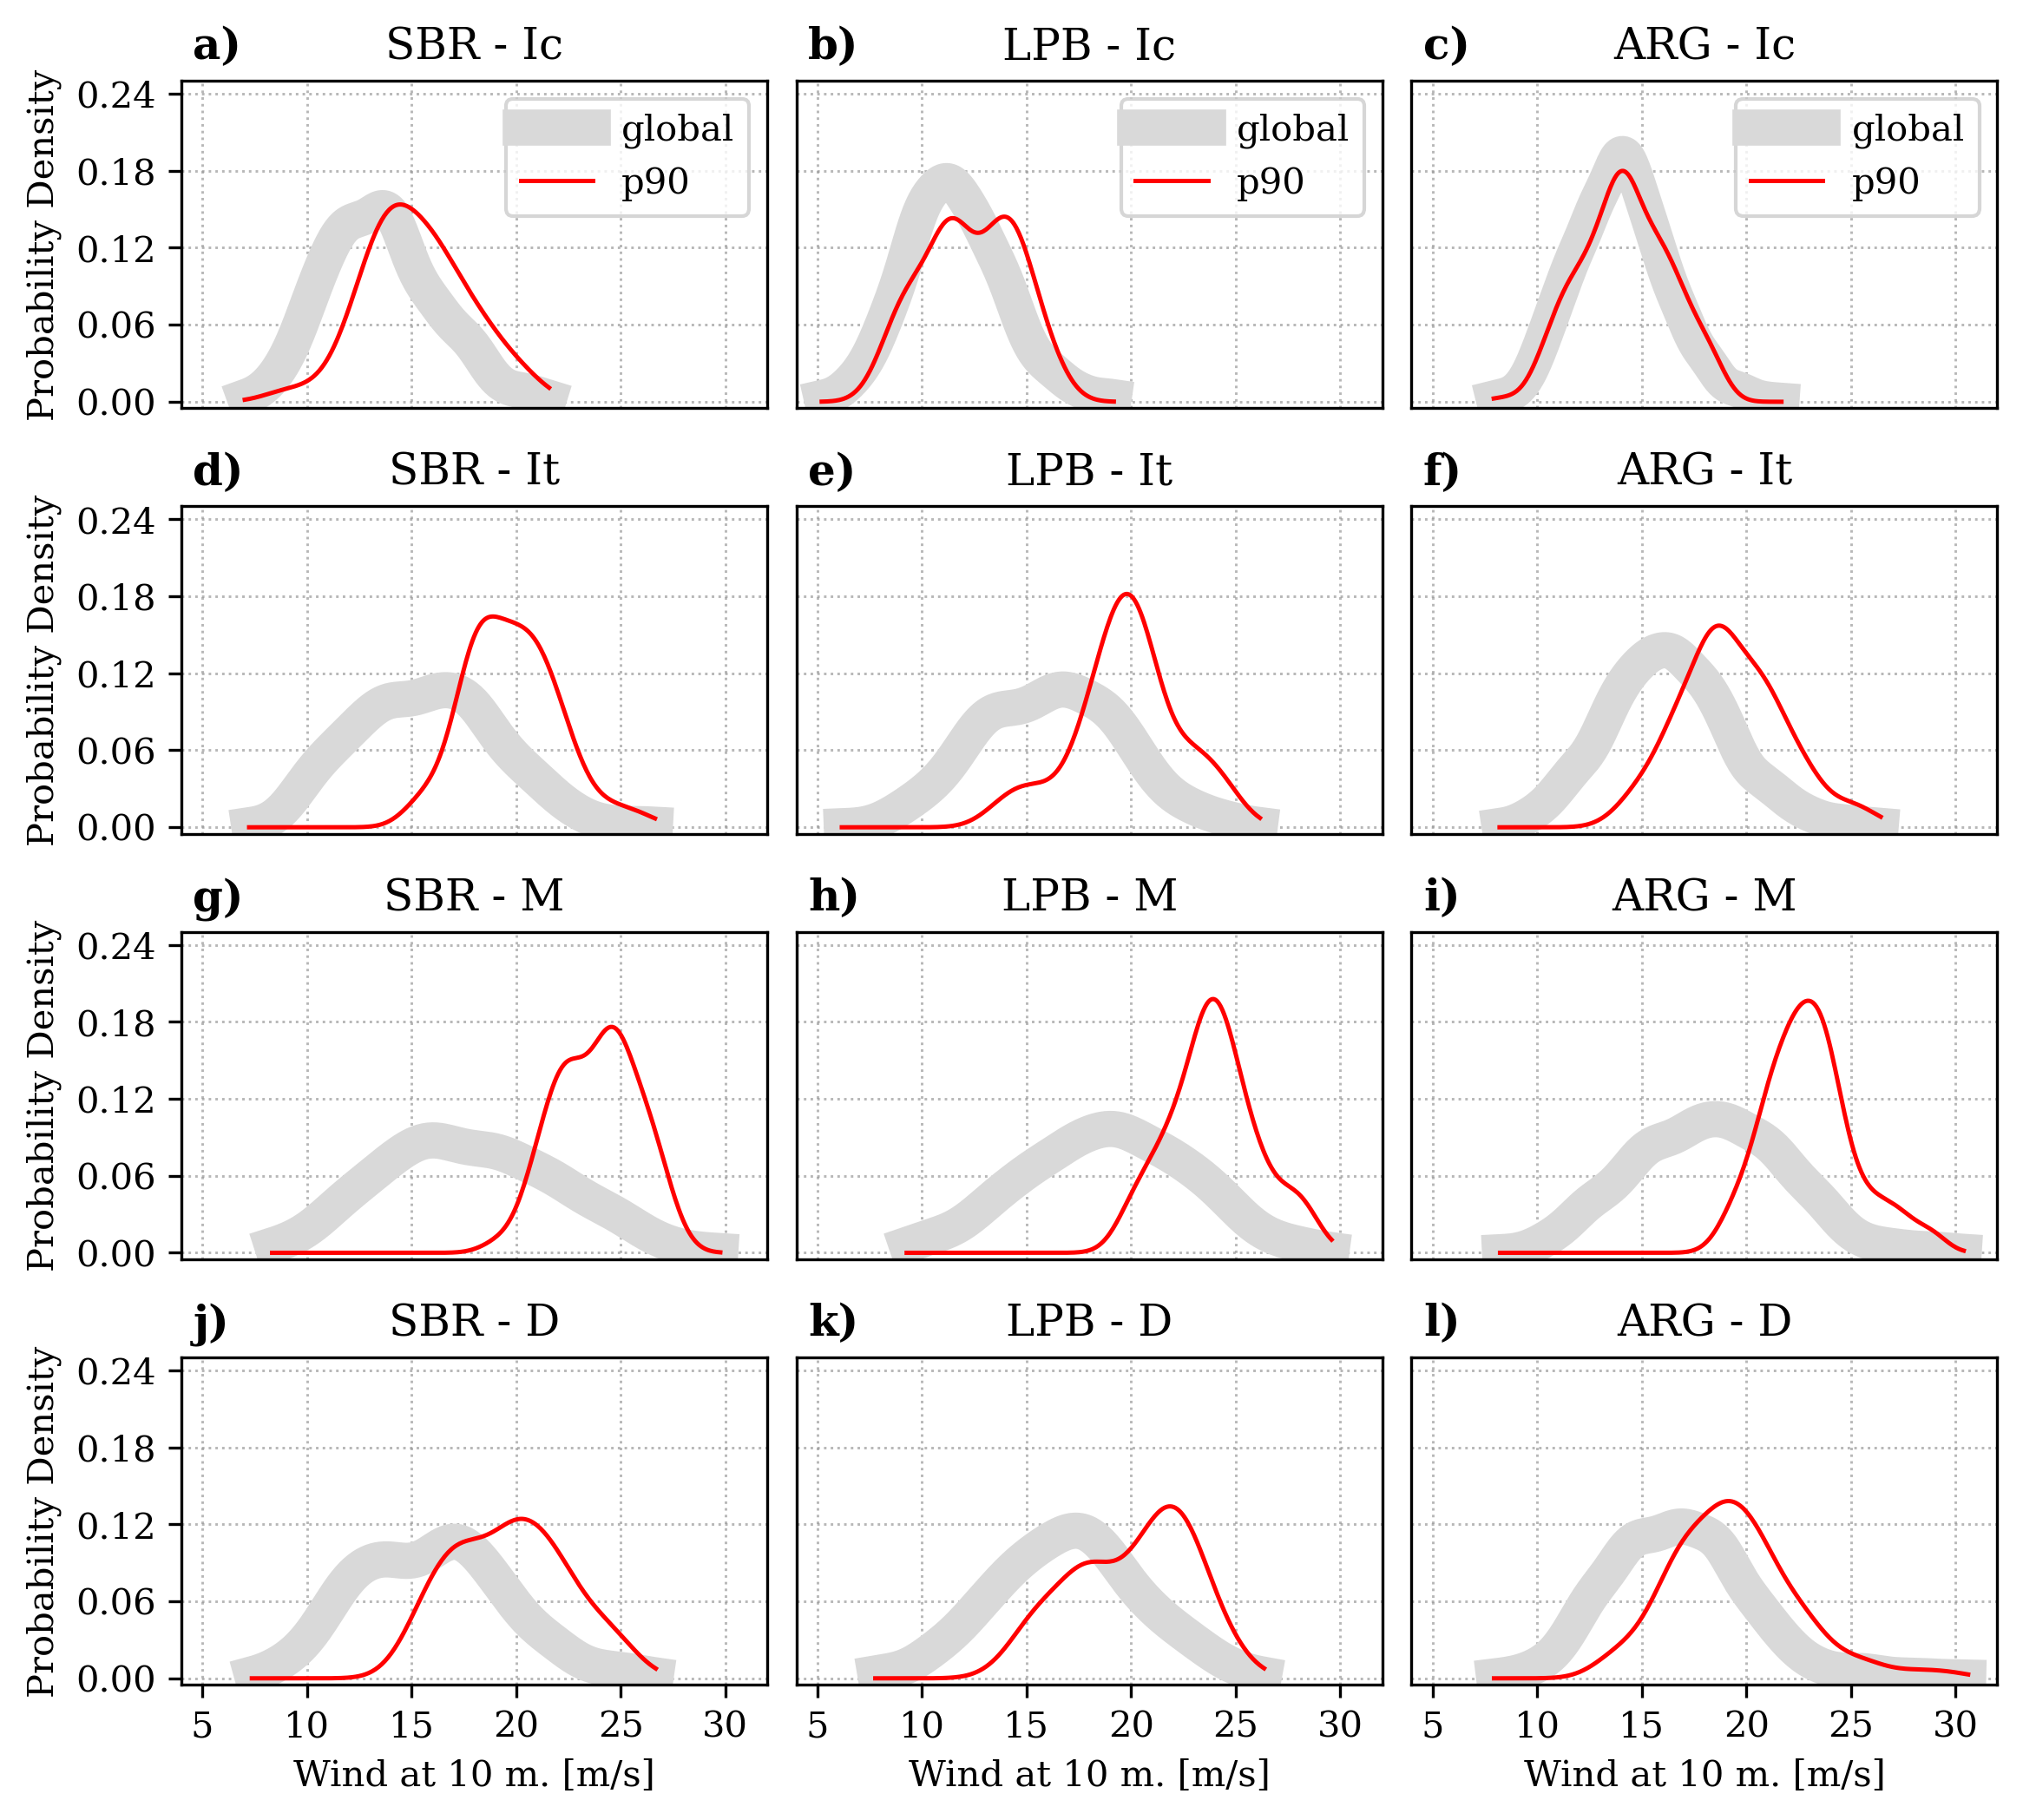
\includegraphics[width=\textwidth]{images/w10/PDF_wind10_sigma025.png}
\caption[PDF de magnitudes máximas de viento a 10 metros]{Funciones de densidad de probabilidad (PDF) para las magnitudes máximas de viento a 10 metros. Las columnas indican la región de ciclogénesis (SBR, LPB, ARG) y las filas la evolución a través de las fases del ciclo de vida (Ic, It, M, D). Se contrasta la población global (referencia, sombreado gris) con los subconjuntos definidos por percentiles de los máximos de vorticidad relativa en 850 hPa alcanzados en su ciclo vital: p10 (sistemas débiles, azul punteado), p50 (sistemas moderados, verde continuo) y p90 (sistemas extremos, rojo seccionado).}
\label{fig:pdf_wind10}
\end{figure}

La Figura \ref{fig:pdf_wind10} presenta un conjunto de funciones de densidad de probabilidad las cuales describen la distribución estadística de los máximos del viento en superficie a 10 metros. Estos valores máximos fueron extraídos del dominio lagrangiano de $20^\circ \times 20^\circ$ centrado en el núcleo de cada sistema. Esta dimensión espacial es consistente con enfoques metodológicos previos aplicados en el Atlántico Sudoccidental, como el de \citet{cardoso2022synoptic}, diseñados específicamente para capturar los vientos extremos que pueden ocurrir a varios cientos de kilómetros del centro del ciclón. La muestra global se encuentra estratificada por región de ciclogénesis (SBR, LPB, ARG) y dividida en subconjuntos de intensidad dinámica definidos según el pico máximo absoluto de vorticidad alcanzado durante todo el ciclo de vida de cada ciclón: sistemas débiles (p10), sistemas moderados (p50) y eventos extremos (p90). Transversalmente, la evolución de estos grupos estáticos se evalúa a lo largo de las cuatro fases de desarrollo (Ic, It, M, D).
% CITA TEXTUAL CARDOSO (2022): [Pega aquí la frase exacta de Cardoso sobre la justificación del radio de captura o el uso de dominios amplios para evaluar la estructura de los ciclones en nuestra región]

Durante la fase incipiente (Ic; paneles a, b y c), las distribuciones para todos los estratos de intensidad presentan una morfología unimodal estrecha y altamente superpuesta, con frecuencias máximas concentradas en el rango de 10 a 17 m/s. A medida que los sistemas evolucionan independientemente hacia las fases de intensificación (It; paneles d, e y f) y madurez (M; paneles g, h e i), se hace evidente la divergencia entre los grupos: la curva del subconjunto extremo (p90) se desplaza drásticamente hacia la derecha, alcanzando en la fase M un pico modal en el rango de 20 a 25 m/s y colas extendiéndose hasta los 30 m/s. Este comportamiento lo distancia claramente de la curva moderada (p50), que mantiene su máximo alrededor de los 15 a 17 m/s, solapándose frecuentemente con la población de referencia. Regionalmente, en la etapa de madurez de SBR (g) y LPB (h), el p90 exhibe picos de densidad agudos (valores de $\sim$0.18) y acotados en altas velocidades, mientras que ARG (i) muestra una distribución p90 más ancha y aplanada, evidenciando una mayor heterogeneidad en la intensidad de sus sistemas extremos. Finalmente, en la fase de decaimiento (D; paneles j, k y l), las curvas p90 retroceden levemente hacia magnitudes menores y aumentan su dispersión, preservando no obstante una separación inconfundible respecto a los sistemas más débiles.

La máxima separación de las distribuciones en la fase de madurez refleja el momento en que los ciclones expresan su pleno potencial dinámico, alcanzando su mínimo absoluto de vorticidad relativa a 850 hPa y maximizando el gradiente horizontal de presión superficial. La marcada diferencia del subconjunto p90 evidencia que estos vórtices poseen, desde su génesis, un entorno o forzante más inestable que culmina en campos de viento sustancialmente más severos que un desarrollo estándar. 
%%
Las variaciones interregionales reflejan distintos forzamientos físicos predominantes. Tal como sostiene \citet{gramcianinov2024early}, los sistemas en las regiones SBR y LPB alcanzan intensidades de viento más extremas debido a la fuerte influencia de procesos termodinámicos en niveles bajos —como la advección cálida y la convergencia de humedad de origen oceánico y continental—, factores que los modelos de alta resolución logran representar con mayor fidelidad. Esta dependencia termodinámica se ilustra en el análisis del ciclón Raoni realizado por \citet{reboita2022from}, donde se evidenció que los flujos turbulentos de calor sensible y latente desde el océano, junto con el transporte de humedad continental por vientos, fueron decisivos para fortalecer el sistema y organizar la convección. Asimismo, experimentos numéricos confirman que la representación precisa de estos intercambios de calor en superficie es esencial para capturar la intensificación de los vientos en niveles bajos. Este aspecto termodinámico es estudiado por \citet{russo2025impacts}, quienes demuestran que la inyección masiva de humedad y flujos de calor latente concentra la energía cinética y favorece el desarrollo baroclínico de sistemas severos.
% REFERENCIA TEXTUAL 
% "gramcianinov2024early The GCMs tend to underestimate the wind intensity in all regions... The RCMs are generally closer to the ERA5 wind speed distribution but with an overestimation of the cyclones' winds, as depicted by the high probability in the right-hand tail".
% RUSSO ET AL. (2025): "The results indicate that latent heat flux associated with SST plays a fundamental role in baroclinic development... Specific humidity in the warm sector was a crucial factor in the intensification of all the cases studied."
Mientras tanto, en ARG, la dinámica baroclínica clásica del frente polar y la perturbación topográfica de los Andes generan respuestas cinemáticas más variables y distribuciones más aplanadas. De acuerdo con \citet{gan1994influence}, la cordillera induce severas distorsiones espaciales en el flujo de niveles bajos, mientras que \citet{vera2002cold} detallan la profunda modificación en la estructura tridimensional de las ondas al cruzar el relieve andino. Esta modulación orográfica explica la mayor heterogeneidad e irregularidad geométrica en el campo de vientos superficiales para los sistemas generados en esta región.
% REFERENCIA TEXTUAL GAN Y RAO (1994): "When the wave approaches the Andes Cordillera, it exhibits orographic effects such as anticyclonic turning of a low-level disturbance trajectory, a zonal trajectory in the upper levels, distortions of the isolines of correlation, and an elongation of maximum correlation on the lee side of the Andes."
% REFERENCIA TEXTUAL VERA ET AL. (2002): "Both cyclonic and anticyclonic perturbations display significant modifications in their three-dimensional structure as they evolve over extratropical and subtropical South America."
La cuantificación de estas distribuciones permite comparar objetivamente cómo evolucionan las magnitudes más probables y la extensión de los valores extremos entre ciclones de distinta génesis. Al confirmar que los ciclones clasificados dinámicamente como extremos (p90) se separan sistemáticamente de la población a medida que maduran, se valida la pertinencia de la clasificación basada en vorticidad. En la fase de madurez, mientras que la moda de los sistemas débiles (p10) se sitúa en torno a los 12-15 m/s, el grupo p90 desplaza su mayor probabilidad hacia los 22 m/s, lo que representa un incremento de aproximadamente el 50\% en la intensidad del viento más frecuente. Las colas en las distribuciones p90 alcanzan magnitudes críticas de hasta 30 m/s. Este corrimiento coincide con los registros documentados por \citet{padilhareinke2026characterization} y \citet{gramcianinov2020analysis} para los eventos severos del Atlántico Sur. \citet{padilhareinke2026characterization} reportan una intensidad media de viento a 10 metros de 70.0 km/h ($\approx$ 19.4 m/s), con un umbral para eventos intensos (p90) de 84.4 km/h ($\approx$ 23.4 m/s) y magnitudes extremas que alcanzan hasta 113.21 km/h ($\approx$ 31.4 m/s) en las colas de la distribución. En una línea complementaria, \citet{gramcianinov2020analysis} documentan, para el invierno austral (JJA), velocidades máximas medias de entre 21.2 ± 4.8 m/s y 23.4 ± 4.8 m/s, con valores del percentil 90 de entre 27.3 y 30.2 m/s y del percentil 95 de hasta 32.1 m/s en bases de datos de alta resolución como CFSR/CFSv2. Desde una perspectiva analítica, lo observado en el Hemisferio Norte por \citet{corner2025classification}, quienes emplean un método de clasificación de ciclones distinto, se identifica que el grupo de los ciclones más débiles presenta una moda en la velocidad del viento a 10 metros de 12.5 m/s. En contraste, ciclones más intensos alcanzan los 22.5 m/s. Las colas en las distribuciones de este grupo extremo alcanzan magnitudes críticas de hasta 35 m/s, lo que confirma que estos sistemas mantienen consistentemente sus valores de viento por encima del umbral de los 20 m/s.
%
Como subraya \citet{gramcianinov2023impact}, identificar tempranamente sistemas extremos resulta indispensable, ya que estos vientos anómalos son los forzantes primarios en la generación de oleaje destructivo y suponen un riesgo directo para las regiones costeras y marítimas.
% CITA TEXTUAL GRAMCIANINOV (2023): "Explosive cyclones over the South Atlantic show highly localized extreme wind cores, which are the primary drivers for the generation of severe wave events."

% ==============================================================================
% SECCIÓN PRINCIPAL: KDE ESPACIAL DE VIENTO A 10 METROS
% ==============================================================================
%
\section{PDF espacial de máximos de viento a 10 metros: Población global}\label{sec:kde_espacial_global}

\begin{figure}[htbp]
\centering
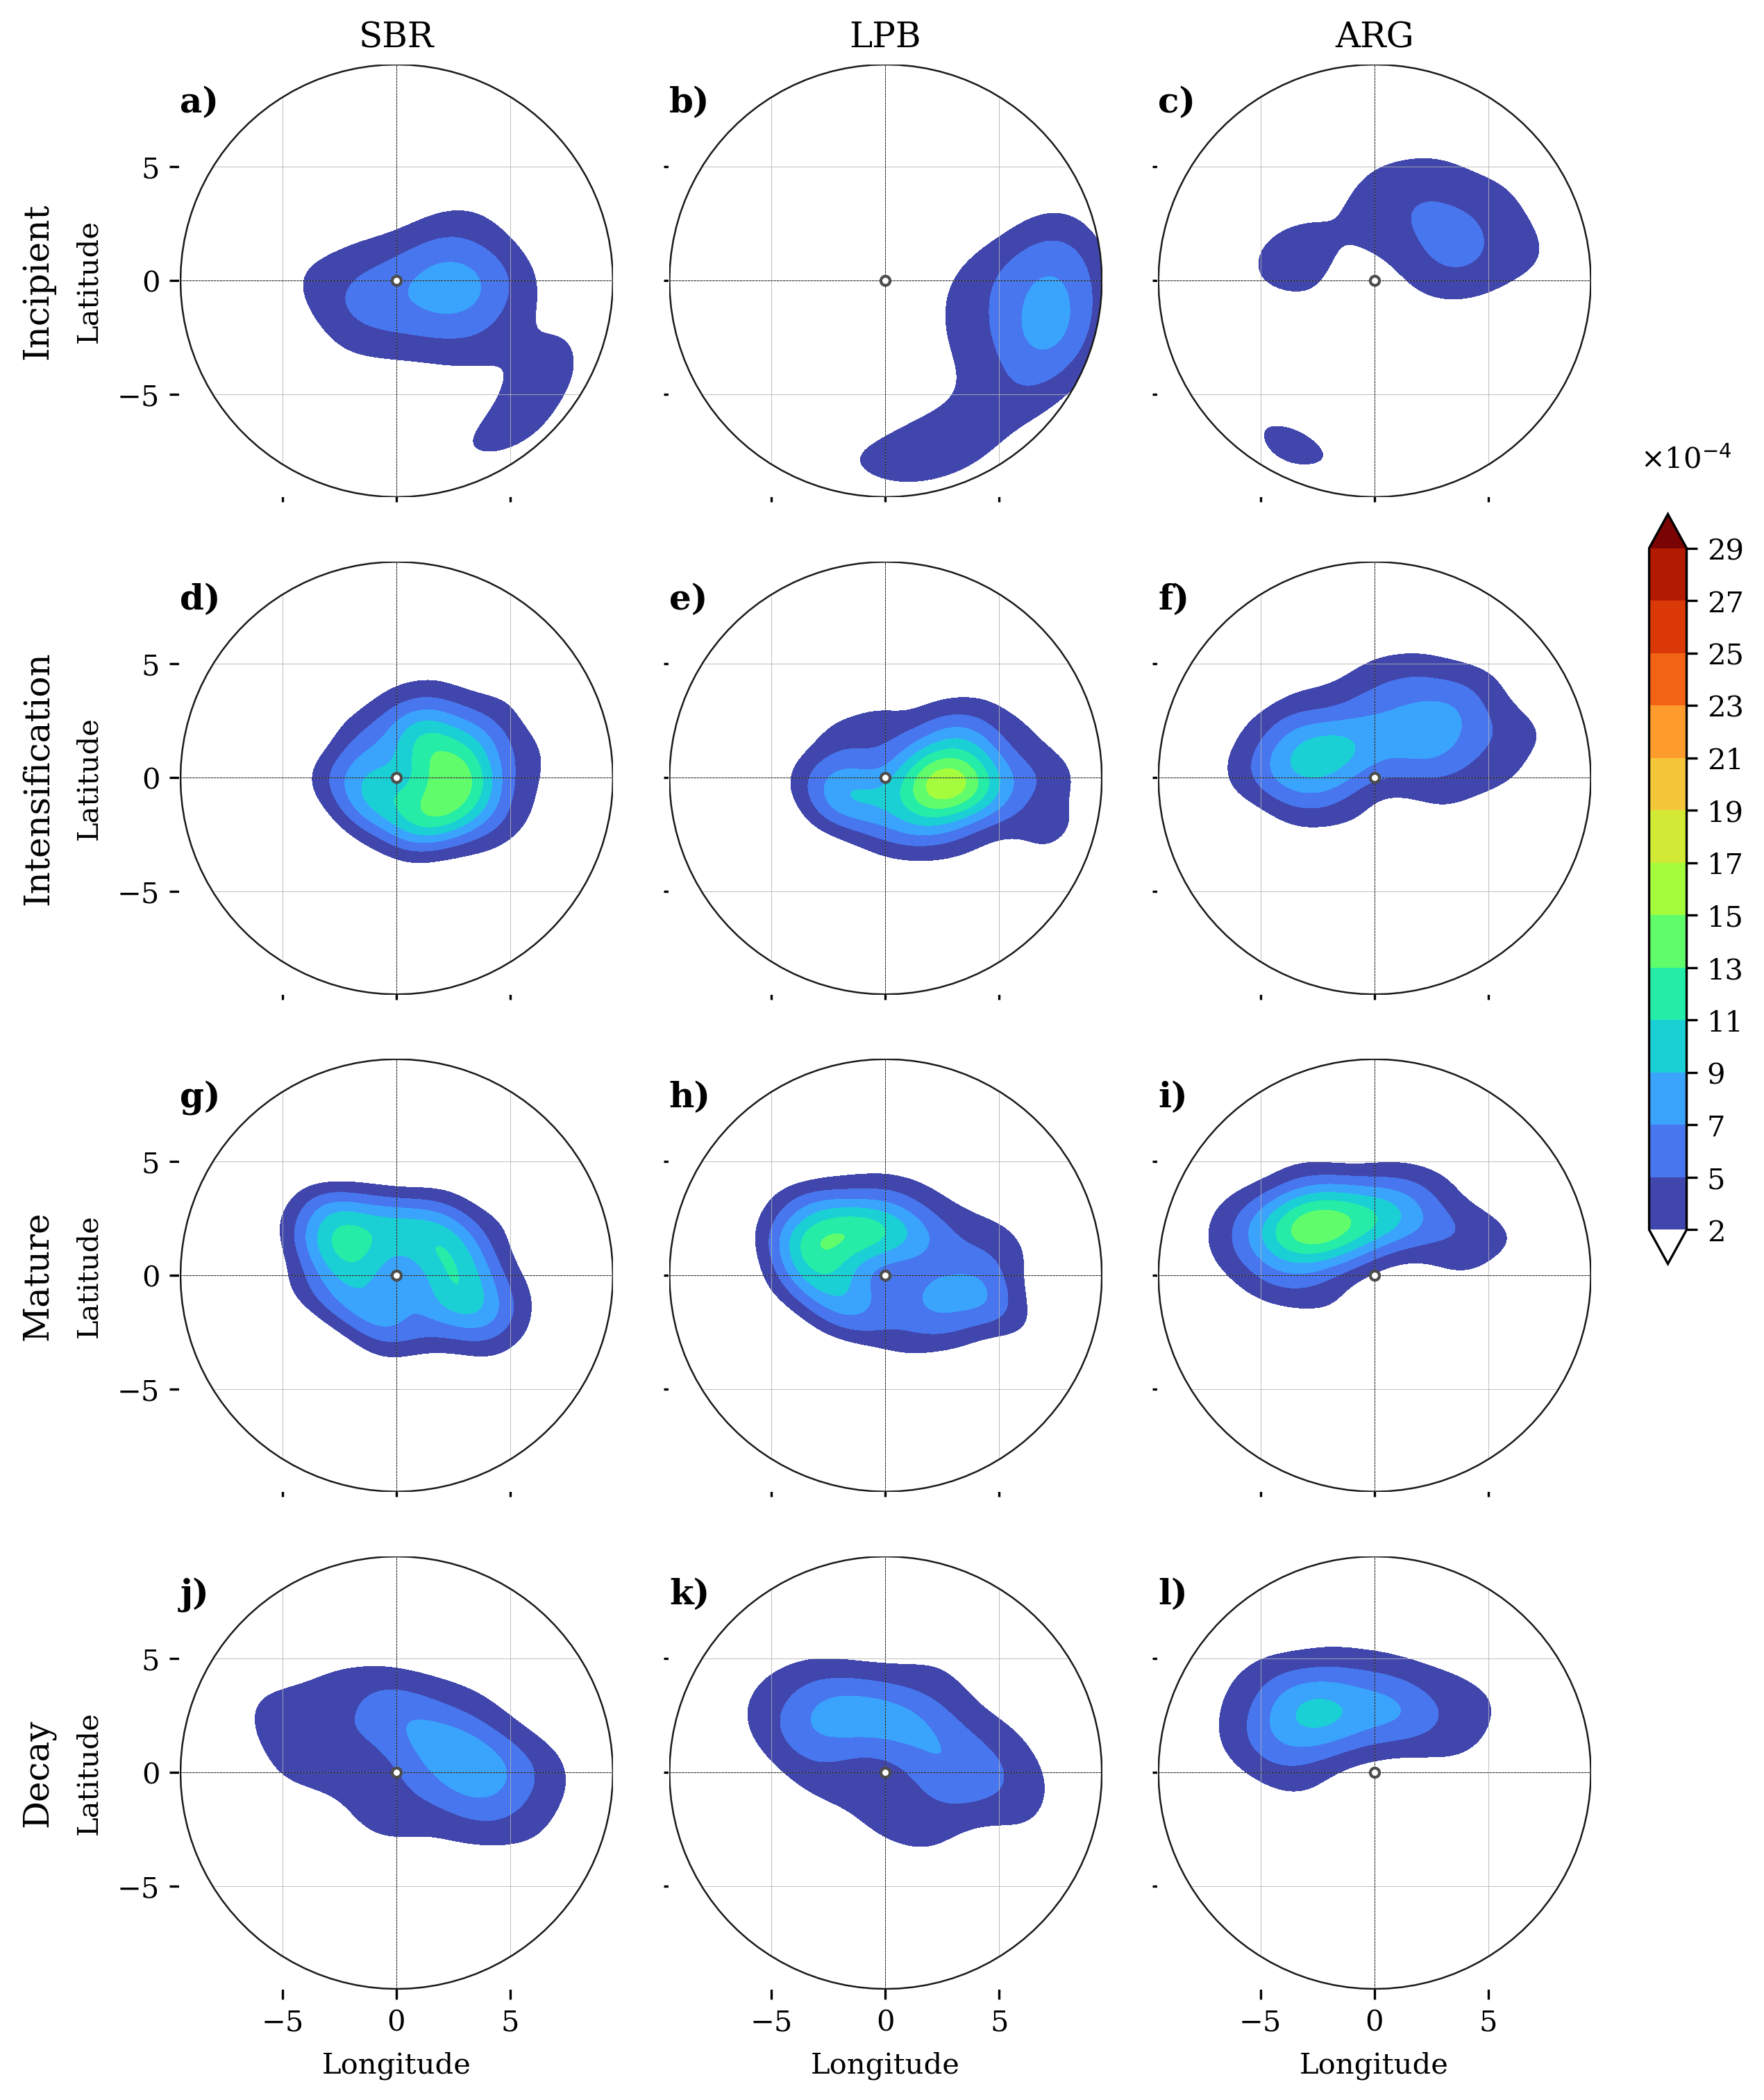
\includegraphics[width=\textwidth]{images/w10/kde_wind10_global_fasesxreg.png}
\caption[PDF espacial de viento máximo a 10 metros - Población Global]{Estimación de densidad espacial bidimensional de la ubicación de los máximos de magnitud de viento a 10 metros para la Población Global. Las columnas separan las regiones de ciclogénesis (SBR, LPB, ARG) y las filas indican las fases evolutivas (Ic, It, M, D). El dominio lagrangiano está centrado en el ciclón ($0^\circ, 0^\circ$).}
\label{fig:kde_wind_global}
\end{figure}

% ¿Qué es?
La Figura \ref{fig:kde_wind_global} presenta el campo de densidad (PDF) espacial de la ubicación geográfica relativa donde se registra el viento máximo a 10 metros. Este análisis corresponde a la Población Global, evaluando todos los ciclones extratropicales del catálogo sin discriminar por su intensidad de la vorticidad relativa. El mapeo probabilístico se estructura sobre un dominio de coordenadas relativas centrado en el núcleo y evalúa la evolución espacial a lo largo de las cuatro fases de vida para las tres regiones de ciclogénesis.

A nivel global, la distribución espacial del máximo de viento se caracteriza por ser amplia, difusa y con gradientes de probabilidad suaves. Las zonas de máxima densidad (tonos amarillos y verdes tenues) abarcan áreas extensas que, en las fases iniciales (Ic; paneles a, b y c), no definen una estructura simétrica alrededor del centro del ciclón en las tres regiones de ciclogénesis. Esta falta de organización inicial concuerda con lo expuesto por \citet{reboita2010south} y \citet{gozzo2017climatology}, quienes señalan la alta variabilidad de los sistemas que componen la población general, incluyendo una abundante ocurrencia de ciclones débiles o someros cuya circulación no logra consolidar un patrón simétrico de vientos en sus primeras etapas.
% CITA TEXTUAL Gozzo et al. (2014/2017): "the abundant occurrence of shallow cyclonic systems, especially near the southeastern Brazilian coast, that do not reach sustained winds of 17 m s-1 but may cause notable weather events"
% CITA TEXTUAL Reboita et al. (2010): "Considering the systems initiate with [weaker vorticity -1.5 x 10(-5) s(-1)], the annual cycle is not well defined... The stronger systems [...] have a well-characterized high frequency"
A medida que el ciclón avanza hacia la madurez (M; paneles g, h e i), se observa una leve preferencia de localización en los cuadrantes del norte y oeste, pero manteniendo diferencias posicionales entre las regiones. Como sugiere \citet{dossantos2023response}, esta evolución espacial asimétrica hacia la madurez está ligada a las zonas baroclínicas, donde los máximos gradientes térmicos horizontales interactúan con los chorros en la alta troposfera.
% CITA TEXTUAL dos Santos et al. (2023): "This type of instability occurs at medium latitudes, in the so-called baroclinic zones, where the maximum horizontal temperature gradients are located on a large scale and where jets are consequently observed in the upper troposphere."
En la etapa de madurez, la densidad máxima en ARG (i) supera valores de $10 \times 10^{-4}$, mientras que SBR (g) y LPB (h) alcanzan una mayor densidad de sus máximos en un área más restringida; esto indica que, en estas dos regiones, existe un foco más recurrente y definido para la localización de los vientos máximos en comparación con la mayor dispersión observada en ARG. De acuerdo con \citet{gramcianinov2019properties} y \citet{cardoso2022synoptic}, este contraste regional responde a los distintos forzantes: mientras que los sistemas en ARG están modulados principalmente por la advección térmica, la mayor concentración y coherencia en SBR y LPB se ve favorecida por la advección de aire cálido y húmedo junto al desarrollo de bajas orográficas en sus etapas iniciales.
% CITA TEXTUAL Gramcianinov et al. (2019): "The cyclone composites reveal that SE-BR [SBR] and SE-SAO cyclones are associated with secondary development, the LA PLATA [LPB] cyclones development is influenced by an orographic low in their early stages, and ARG cyclones are influenced by thermal advection as an essential mechanism in the reduction of static stability."
% CITA TEXTUAL Gramcianinov et al. (2019): "The increase in genesis at 30S over the continent is associated with the strengthening of the upper-level jet and the increase of warm and moisture advections at the same location."

%%%%%%
%%%%
%%%%
Esta alta dispersión y baja coherencia espacial es el resultado de utilizar un catálogo masivo donde los sistemas varían desde configuraciones débiles hasta atípicas. Como señala \citet{sinclair1994objective}, los métodos de identificación y seguimiento basados en vorticidad capturan un espectro mucho más amplio de sistemas, incluyendo numerosos ciclones débiles, móviles y de menor duración que presentan una gran variabilidad en su intensidad, configuración frontal y trayectoria. Físicamente, en sistemas con un forzante dinámico débil, el flujo sinóptico de niveles medios o altos domina la circulación y limita su intensidad, desplazamiento y duración. De acuerdo con \citet{hoskins2005new}, cuando la interacción baroclínica es débil, el sistema es gobernado principalmente por anomalías en la alta troposfera que no logran consolidar un acoplamiento profundo, lo que modifica la ubicación del viento máximo en niveles bajos en función de gradientes de presión transitorios y menos anclados a la dinámica interna del ciclón.
% CITA TEXTUAL Sinclair (1994): "The vorticity-based climatology includes many more weak, mobile, and short-lived weather systems than are found from MSLP analyses."
% CITA TEXTUAL Hoskins y Hodges (2005): "In the absence of strong baroclinic development, upper-tropospheric features can exist and propagate without a significant low-level signature [...] leading to a weaker coupling." (Basado en la discusión sobre el desarrollo baroclínico y la propagación de anomalías de PV en niveles altos frente a la vorticidad en niveles bajos).

La caracterización de la Población Global es esencial porque establece la línea base de dispersión espacial. Al demostrar que en un conjunto general el máximo de viento puede ocurrir en un radio muy amplio y variable, se justifica la necesidad metodológica de estratificar la muestra por intensidad. Esta necesidad de clasificar las bases de datos masivas es fuertemente respaldada por investigaciones recientes desarrolladas para el Hemisferio Norte, como las de \citet{corner2025classification} y \citet{eisenstein2023identification}. Estos autores destacan que la diversidad de estos sistemas exige clasificarlos para aislar los eventos severos. Aunque esta estratificación ya es habitual en el Hemisferio Norte, su aplicación sistemática en el Hemisferio Sur sigue siendo una necesidad crítica. Así, este mapa general sirve como línea base para contrastar y cuantificar la organización geométrica de los sistemas más extremos.
% CITA TEXTUAL Corner et al. (2025): "Given the large number and variety of extratropical cyclones, objective classification is necessary to understand their diverse physical characteristics and impacts."
% CITA TEXTUAL Eisenstein et al. (2023): "To fully understand the spectrum of cyclone impacts, it is essential to distinguish between the large number of weak systems and the minority of intense storms that produce severe weather."
%%%%

\section{Distribución espacial de máximos de viento a 10 metros: Subconjunto extremo (p90)}\label{sec:kde_espacial_p90}

\begin{figure}[htbp]
\centering
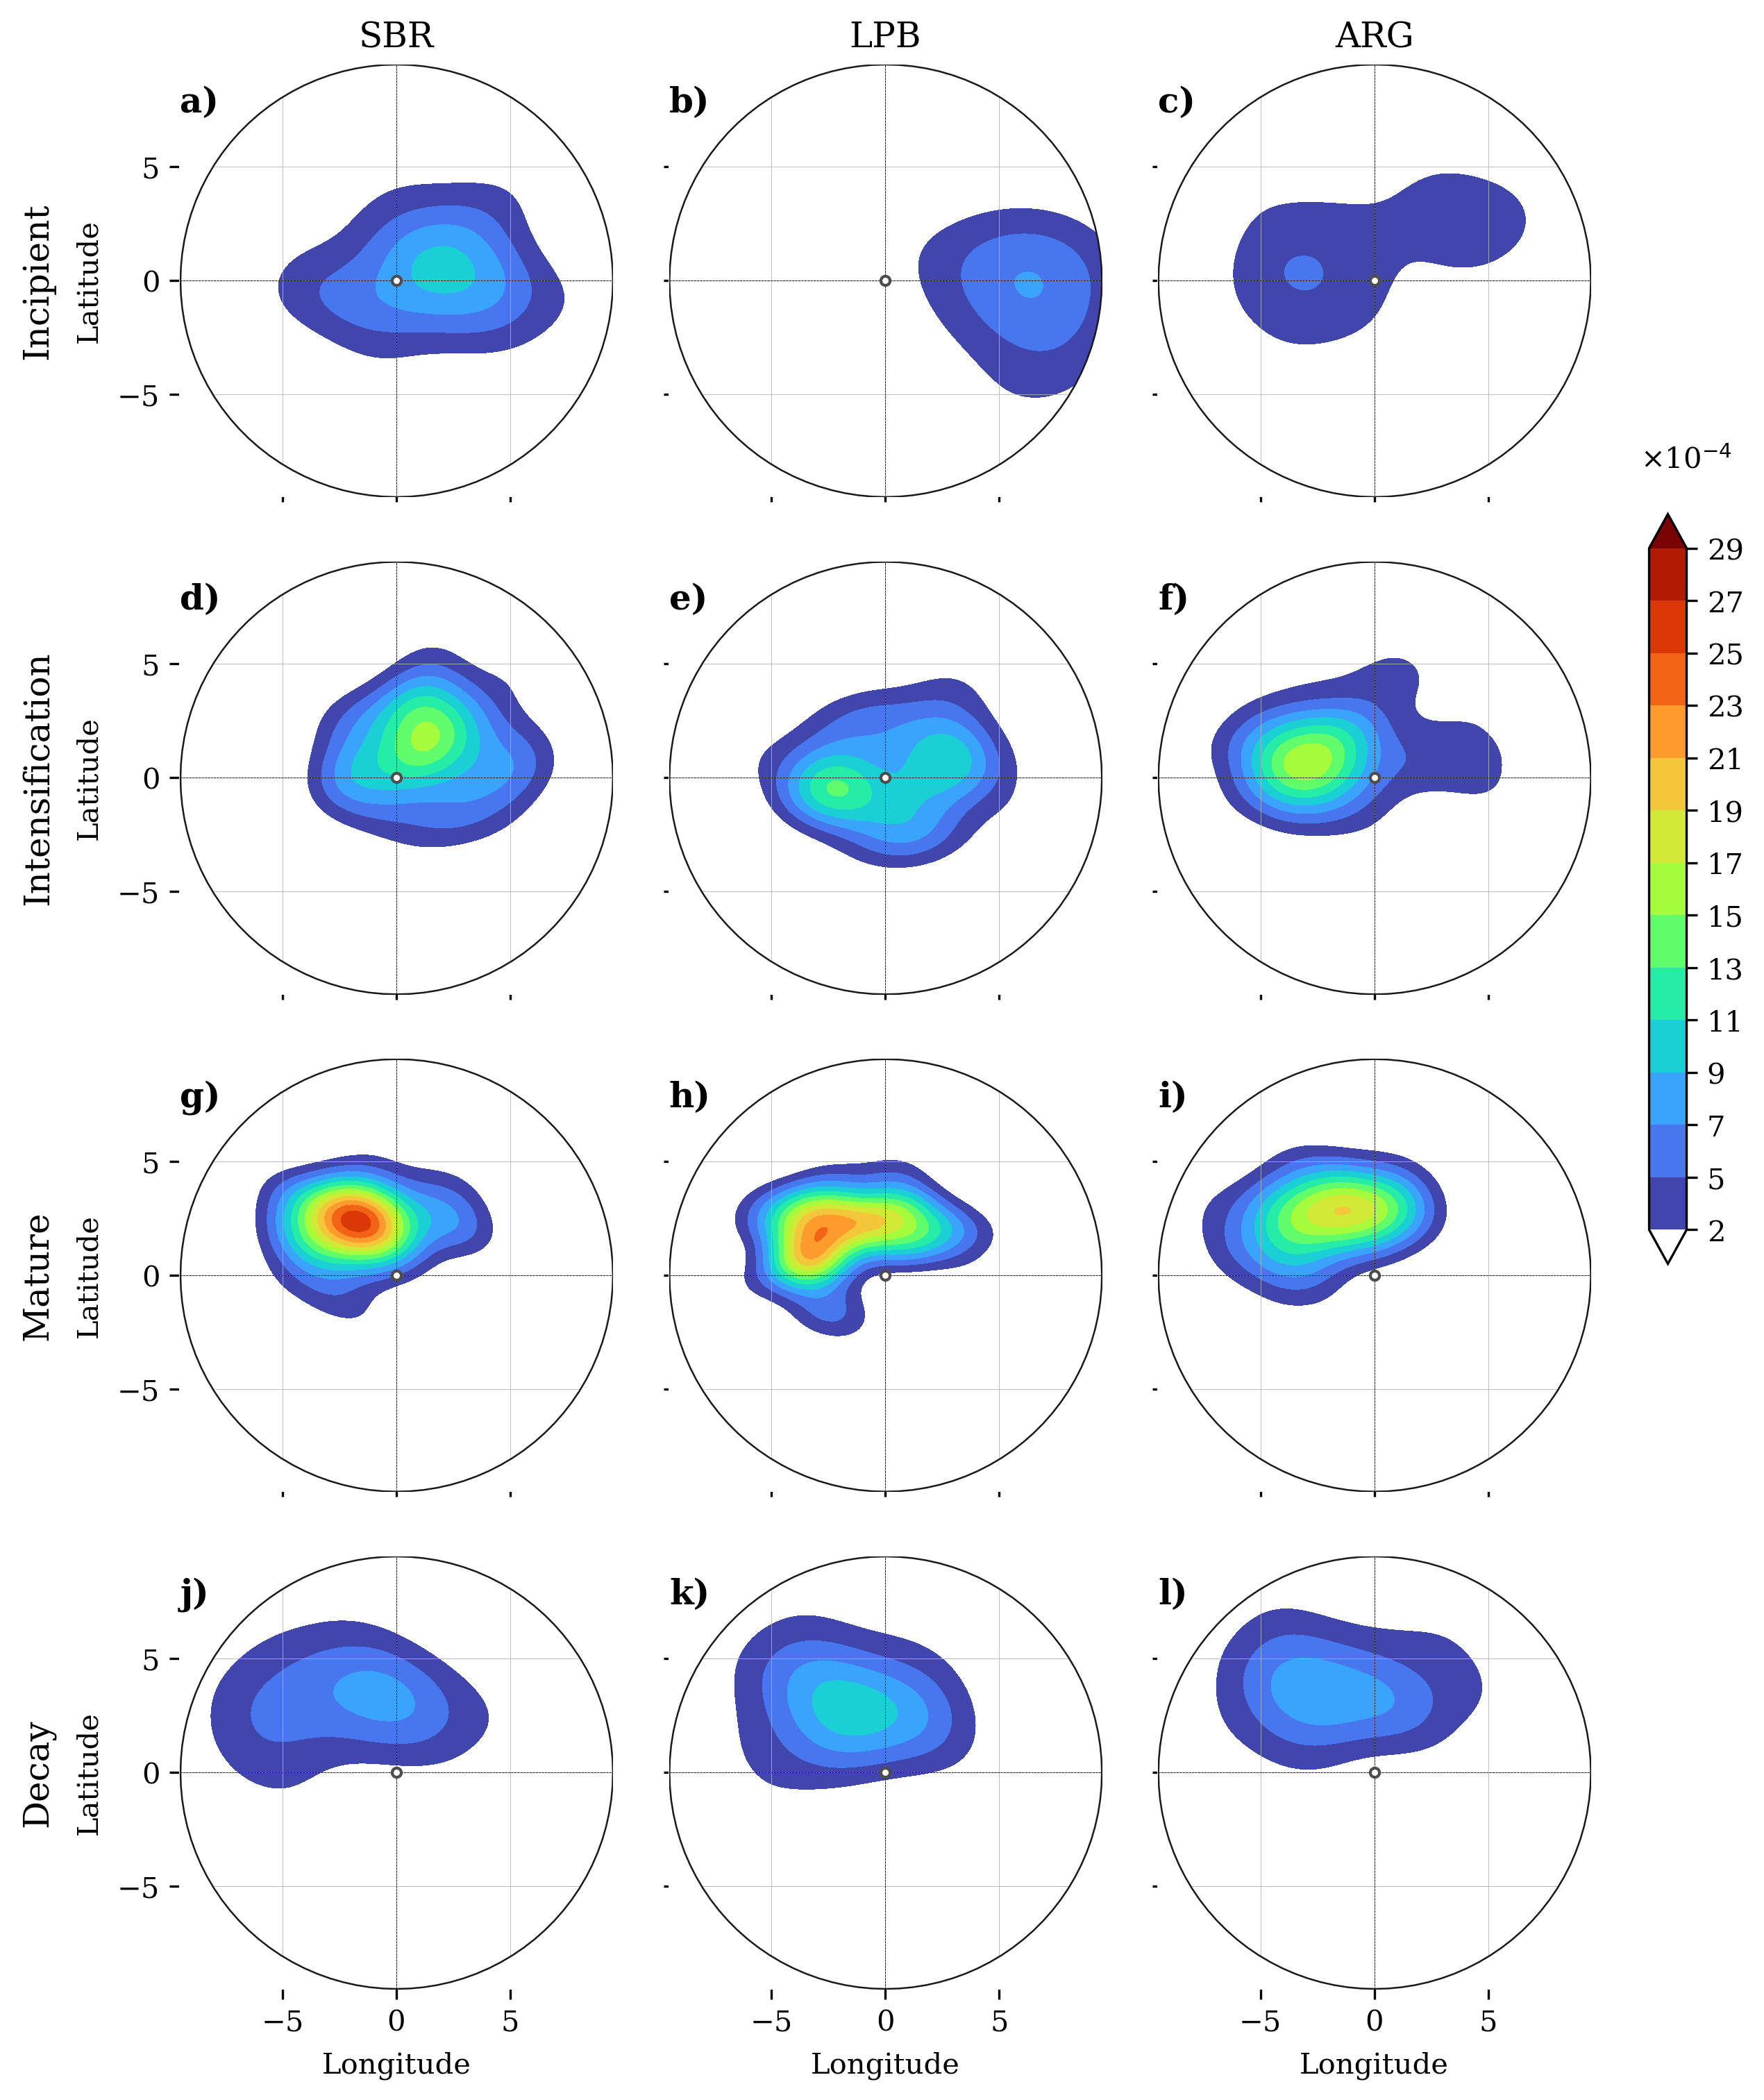
\includegraphics[width=\textwidth]{images/w10/kde_wind10_p90_fasesxreg.png}
\caption[PDF espacial de viento máximo a 10 metros  - Subconjunto p90]{Estimación de densidad espacial bidimensional de la ubicación de los máximos de magnitud de viento a 10 metros para el subconjunto de ciclones intensos. El formato, dominio lagrangiano, fases evolutivas y escala de densidad ($10^{-4}$) son idénticos a los presentados en la Figura \ref{fig:kde_wind_global} para permitir la comparación estructural directa de las asimetrías de densidad.}
\label{fig:kde_wind_p90}
\end{figure}

% ¿Qué es?
La Figura \ref{fig:kde_wind_p90} presenta el campo de densidad (PDF) espacial de la ubicación de los máximos de viento a 10 metros, calculado exclusivamente para el estrato de sistemas extremos (percentil 90). Esta muestra aísla a los vórtices dinámicamente más severos del catálogo, agrupados por haber alcanzado los valores mínimos de vorticidad relativa a 850 hPa dentro del decil de la distribución de menor vorticidad relativa durante el ciclo de vida. Los mapas de densidad correspondientes a los estratos independientes de menor intensidad (sistemas débiles p10 y moderados p50) ilustran el contraste estructural del sistema para los ciclones que alcanzan menores intensidades y se encuentran documentados en el Apéndice \ref{apendice:kde_espacial}.

A diferencia de la dispersión observada en la Población Global (Figura \ref{fig:kde_wind_global}), la arquitectura espacial del estrato p90 exhibe una concentración sustancialmente superior. Al evolucionar hacia la fase de madurez (M; paneles g, h e i), se configura un núcleo de alta densidad en el cuadrante noroeste (aproximadamente a $-3^{\circ}$ de longitud y $+2^{\circ}$ a $+3^{\circ}$ de latitud relativa al centro del ciclón). Las magnitudes de densidad en las regiones SBR (g) y LPB (h) alcanzan el extremo (tonos naranjas y rojos, con valores entre 23 y $29 \times 10^{-4}$), denotando una altísima recurrencia espacial para la localización de los vientos máximos. En contraste, la región ARG (i), aunque marcadamente más concentrada que la muestra global, presenta un núcleo con un aumento de densidad comparativamente menor respecto a SBR y LPB. Al ingresar a la fase de decaimiento (D; paneles j, k y l), el núcleo asimétrico observado en la Población Global altera su posicionamiento hacia el sector noroeste; este cambio es especialmente notorio en SBR (j), donde la mayor densidad en la muestra global se ubicaba previamente en el sector noreste.

El campo de densidad del subconjunto p90 demuestra que los ciclones más profundos poseen, por naturaleza, una ubicación hiperconcentrada de sus vientos máximos en el cuadrante noroeste (Hemisferio Sur) durante su fase madura. Como ha sido documentado para el Hemisferio Norte (cuadrante suroeste) por \citet{clark2005sting} y \citet{han2025system}, los sistemas extratropicales más intensos empaquetan sus vientos extremos en el sector posterior del sistema, específicamente asociados a la zona de fractura frontal y al desarrollo de intensas corrientes en chorro de niveles bajos (como el \textit{sting jet} o la cinta transportadora fría). Al aplicar el efecto espejo producto de la circulación ciclónica inversa entre hemisferios, la configuración dinámica del sector posterior correspondería espacialmente al cuadrante noroeste. Físicamente, la consolidación de este núcleo extremo en superficie responde a procesos de transferencia de cantidad de movimiento. Como sostiene \citet{hyeok2024extrem}, en las inmediaciones del frente frío se desarrollan intensas corrientes descendentes (downdrafts) impulsadas por la convergencia térmica, las cuales transportan el momento horizontal de la alta troposfera hacia la capa límite. No obstante, es preciso señalar que este estudio se centró específicamente en ciclones de latitudes medias del Atlántico Norte. Los resultados revelan que las corrientes descendentes extremas son más frecuentes que los ascensos, aunque este mecanismo depende de la fase del sistema, ya que la superficie frontal no siempre actúa como una barrera efectiva durante las etapas de desarrollo inicial o disipación. Por último, debe considerarse que los datos de reanálisis ERA5 empleados podrían subestimar la intensidad real del viento en superficie debido a limitaciones inherentes a su resolución. Sumado a esto, Gentile et al. (2023) demuestran que los chorros de la cinta transportadora fría (CCBb) en ciclones maduros están asociados con capas límite significativamente más profundas. Esta profundidad, potenciada por la inestabilidad que genera el aire frío al circular sobre aguas oceánicas relativamente más cálidas, induce flujos de calor positivos que facilitan una mezcla vertical descendente altamente eficiente de aire con alta velocidad hacia la superficie. Este proceso se manifiesta en nuestro KDE como un empaquetamiento localizado de vientos a 10 metros, sector donde el CCBb es el principal motor de riesgos de viento a pesar de que modelos como ERA5 tienden a subestimar estas intensidades en aproximadamente un 4.5 m/s.
% CITA TEXTUAL Clark et al. (2005): "The sting jet is a transient mesoscale airflow that descends from the cloud head into the frontal-fracture region, producing damaging surface winds."
% CITA TEXTUAL Han et al. (2025): "For the most intense extratropical cyclones, extreme winds are predominantly associated with the cold conveyor belt and sting jets, concentrating in the rear-left [northwest] quadrant relative to the storm center."
% CITA TEXTUAL Reboita et al. (2018): "Cyclones developing over the western South Atlantic are strongly influenced by the Brazil Current, where sensible and latent heat fluxes contribute significantly to rapid intensification."
% CITA TEXTUAL Gramcianinov et al. (2023): "Explosive cyclones over the South Atlantic show highly localized extreme wind cores, which are the primary drivers for the generation of severe wave events."
Las diferencias interregionales documentadas para el Hemisferio Sur respaldan este marco dinámico. Por un lado, \citet{reboita2018extratropical} destaca que el Atlántico Sudoccidental es un entorno donde las interacciones diabáticas y los fuertes flujos de calor latente océano-atmósfera fomentan la rápida intensificación de los sistemas. Conectando estos procesos térmicos con una zonificación específica, \citet{gramcianinov2023impact} señala que los ciclones originados particularmente en SBR y LPB capitalizan estas condiciones para generar desarrollos de tipo explosivo, empaquetando el momento cinético en un sector espacial muy estrecho. Por el contrario, en ARG, la dinámica baroclínica clásica del frente polar y la perturbación topográfica de los Andes generan estructuras marginalmente más elongadas que dejaran las ubicaciones de los maximos de viento menos concentradas.

La cuantificación de esta concentración responde a un interrogante de esta investigacion, demostrando que el grado de severidad de un ciclón predetermina su patron espacial. Los sistemas extremos originados en el Atlántico Sur concentrarán casi invariablemente sus máximos de viento a 10 metros en un radio y cuadrante particular respecto a su centro. Tal como destaca \citet{dalanhese2023new} para el litoral sudamericano, esta previsibilidad geométrica es una herramienta importante para conocer la espacialidad de las posibles afectaciones que puedan ocurrir durante estos eventos severos.
% CITA TEXTUAL Dalanhese et al. (2023): "Accurate forecasting of the spatial distribution of extreme winds is critical to improve early warning systems and mitigate structural damage to coastal regions in southern Brazil."

% ==============================================================================
% SECCIÓN: PATRONES DOMINANTES DE VARIABILIDAD (EOF) - VIENTO A 10 METROS
% ==============================================================================
\section{Varianza explicada del Viento a 10 metros}\label{sec:var_exp_wind10}

\begin{figure}[!ht]
\centering
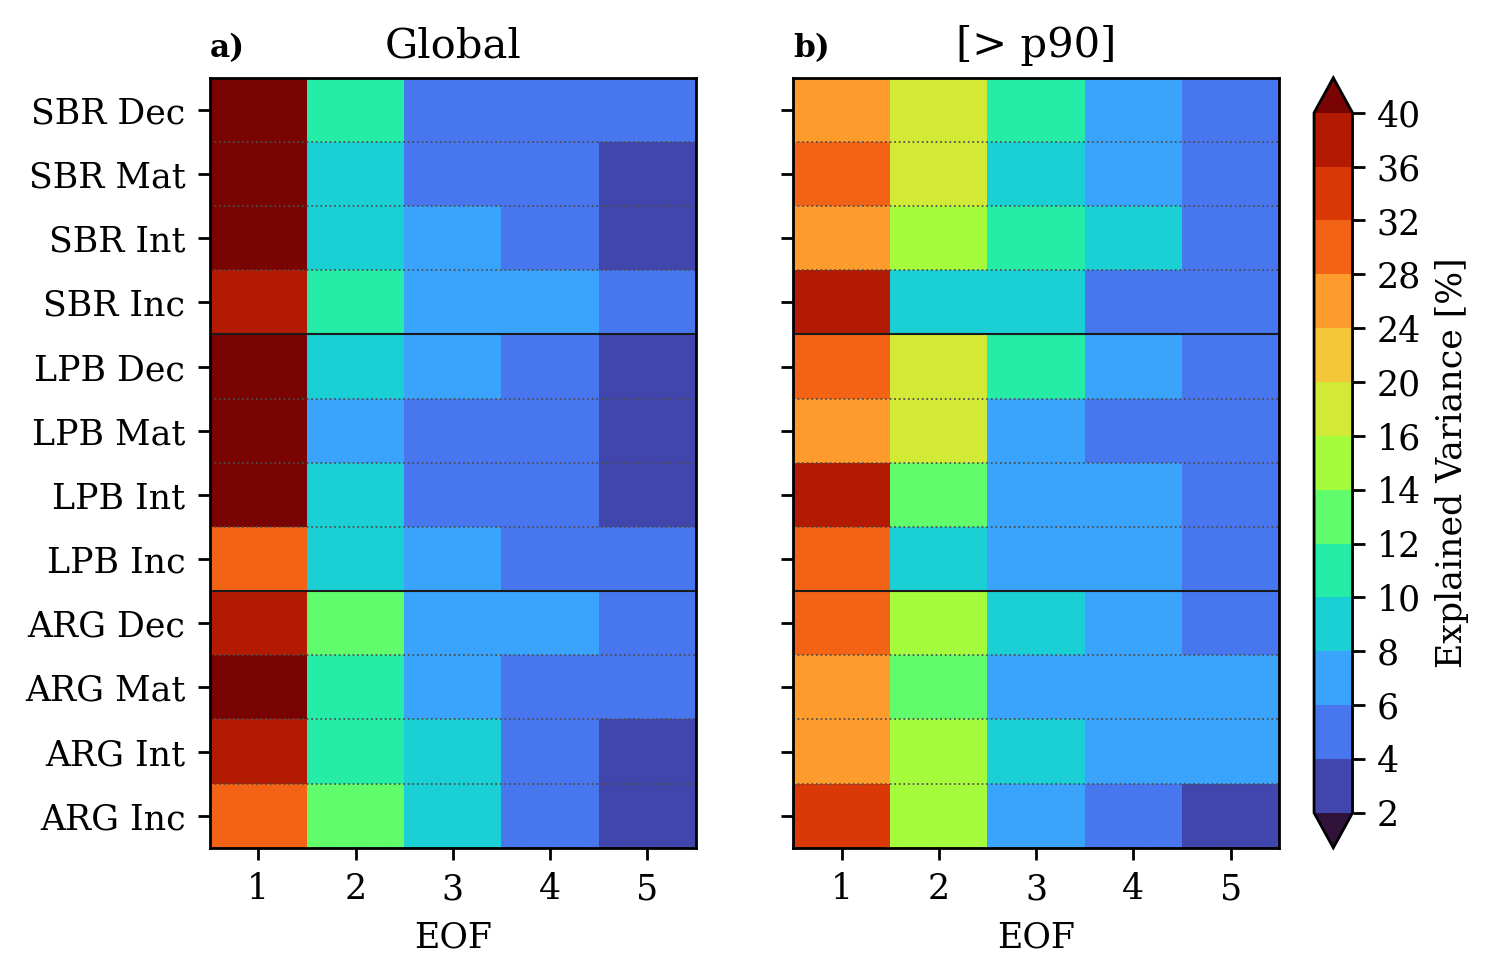
\includegraphics[width=\textwidth]{images/w10/all_expvar_wind10_mean2times.png} 
\caption[Varianza explicada por los primeros cinco modos (EOF1-EOF5) de viento a 10 m]{Fraccionamiento de la varianza espacial total contenida en los primeros cinco modos dominantes (EOF1 a EOF5) del viento a 10 metros. Se contrasta la distribución de la varianza de la Población Global frente a los estratos de intensidad (p10, p50 y p90) a lo largo del ciclo de vida para cada región de ciclogénesis.}
\label{fig:var_exp_wind10}
\end{figure}

% ¿Qué es?
La Figura \ref{fig:var_exp_wind10} sintetiza el fraccionamiento de la varianza espacial distribuida en los primeros cinco modos ortogonales (EOF1 a EOF5) del campo de viento superficial. Este desglose permite evaluar la dimensionalidad y cohesión de la energía cinética. Se contrasta el comportamiento de la Población Global de referencia frente a los estratos de distinta intensidad dinámica intrínseca (p10, p50 y p90) a lo largo de las fases evolutivas.

% ¿Cómo es?
El análisis revela una divergencia drástica en la distribución de la varianza entre las poblaciones. En la Población Global, así como en los estratos de menor y media intensidad (p10 y p50), el modo EOF1 ejerce un dominio abrumador, capturando hasta el 57.1\% (LPB) y el 57.4\% (SBR) de la varianza en la fase de madurez. Esto genera una caída abrupta entre el primer modo y los modos de orden superior (EOF2 a EOF5), los cuales retienen porciones marginales de energía, confirmando que la dinámica de los sistemas p10 y p50 no altera la dimensionalidad base del sistema. Por el contrario, al evaluar el estrato extremo (p90), la concentración de varianza en EOF1 se reduce drásticamente: el EOF1 no logra superar el 37.6\% de representatividad, registrando mínimos de hasta 25.4\% durante la intensificación en ARG. Consecuentemente, la varianza del p90 se reparte y aplana, inflando la importancia relativa de los modos secundarios (EOF2 y EOF3).

% ¿Por qué es así?
La alta concentración de energía en un solo modo (EOF1) para el grupo global, p10 y p50 corrobora que en general los ciclones son gobernados por un gradiente de gran escala impuesto por el flujo sinóptico de fondo. Sin embargo, el aplanamiento de la varianza en los eventos severos (p90) confirma estadísticamente la fragmentación multiescalar. Tal como establece la teoría matemática de \citet{hannachi2007empirical}, un espectro de autovalores más plano es el indicador de que la energía de un sistema complejo se ha distribuido entre múltiples modos competitivos. Al intensificarse, el vórtice extremo genera perturbaciones internas no lineales: frentes excepcionalmente activos, corrientes en chorro de bajos niveles y seclusiones térmicas. Estas estructuras de mesoescala compiten entre sí por la energía cinética del campo, obligando a la descomposición matemática a utilizar múltiples dimensiones ortogonales (EOF2-EOF5) para poder reconstruir el caos cinemático del ciclón.

% ¿Para qué?
Esta métrica constituye una demostración cuantitativa irrefutable de que la severidad extrema no equivale a un simple escalado lineal de un ciclón ordinario. Concluir que los eventos extremos (p90) requieren múltiples dimensiones espaciales para ser explicados es crítico para la modelación numérica: demuestra que parametrizar vientos destructivos asumiendo los patrones simples de la población media subestimará sistemáticamente la agresividad, la naturaleza asimétrica y la localización real de las ráfagas.


\section{Patrones de variabilidad del viento a 10 metros: EOF1 población global}\label{sec:eof1_wind10_global}

\begin{figure}[htbp]
\centering
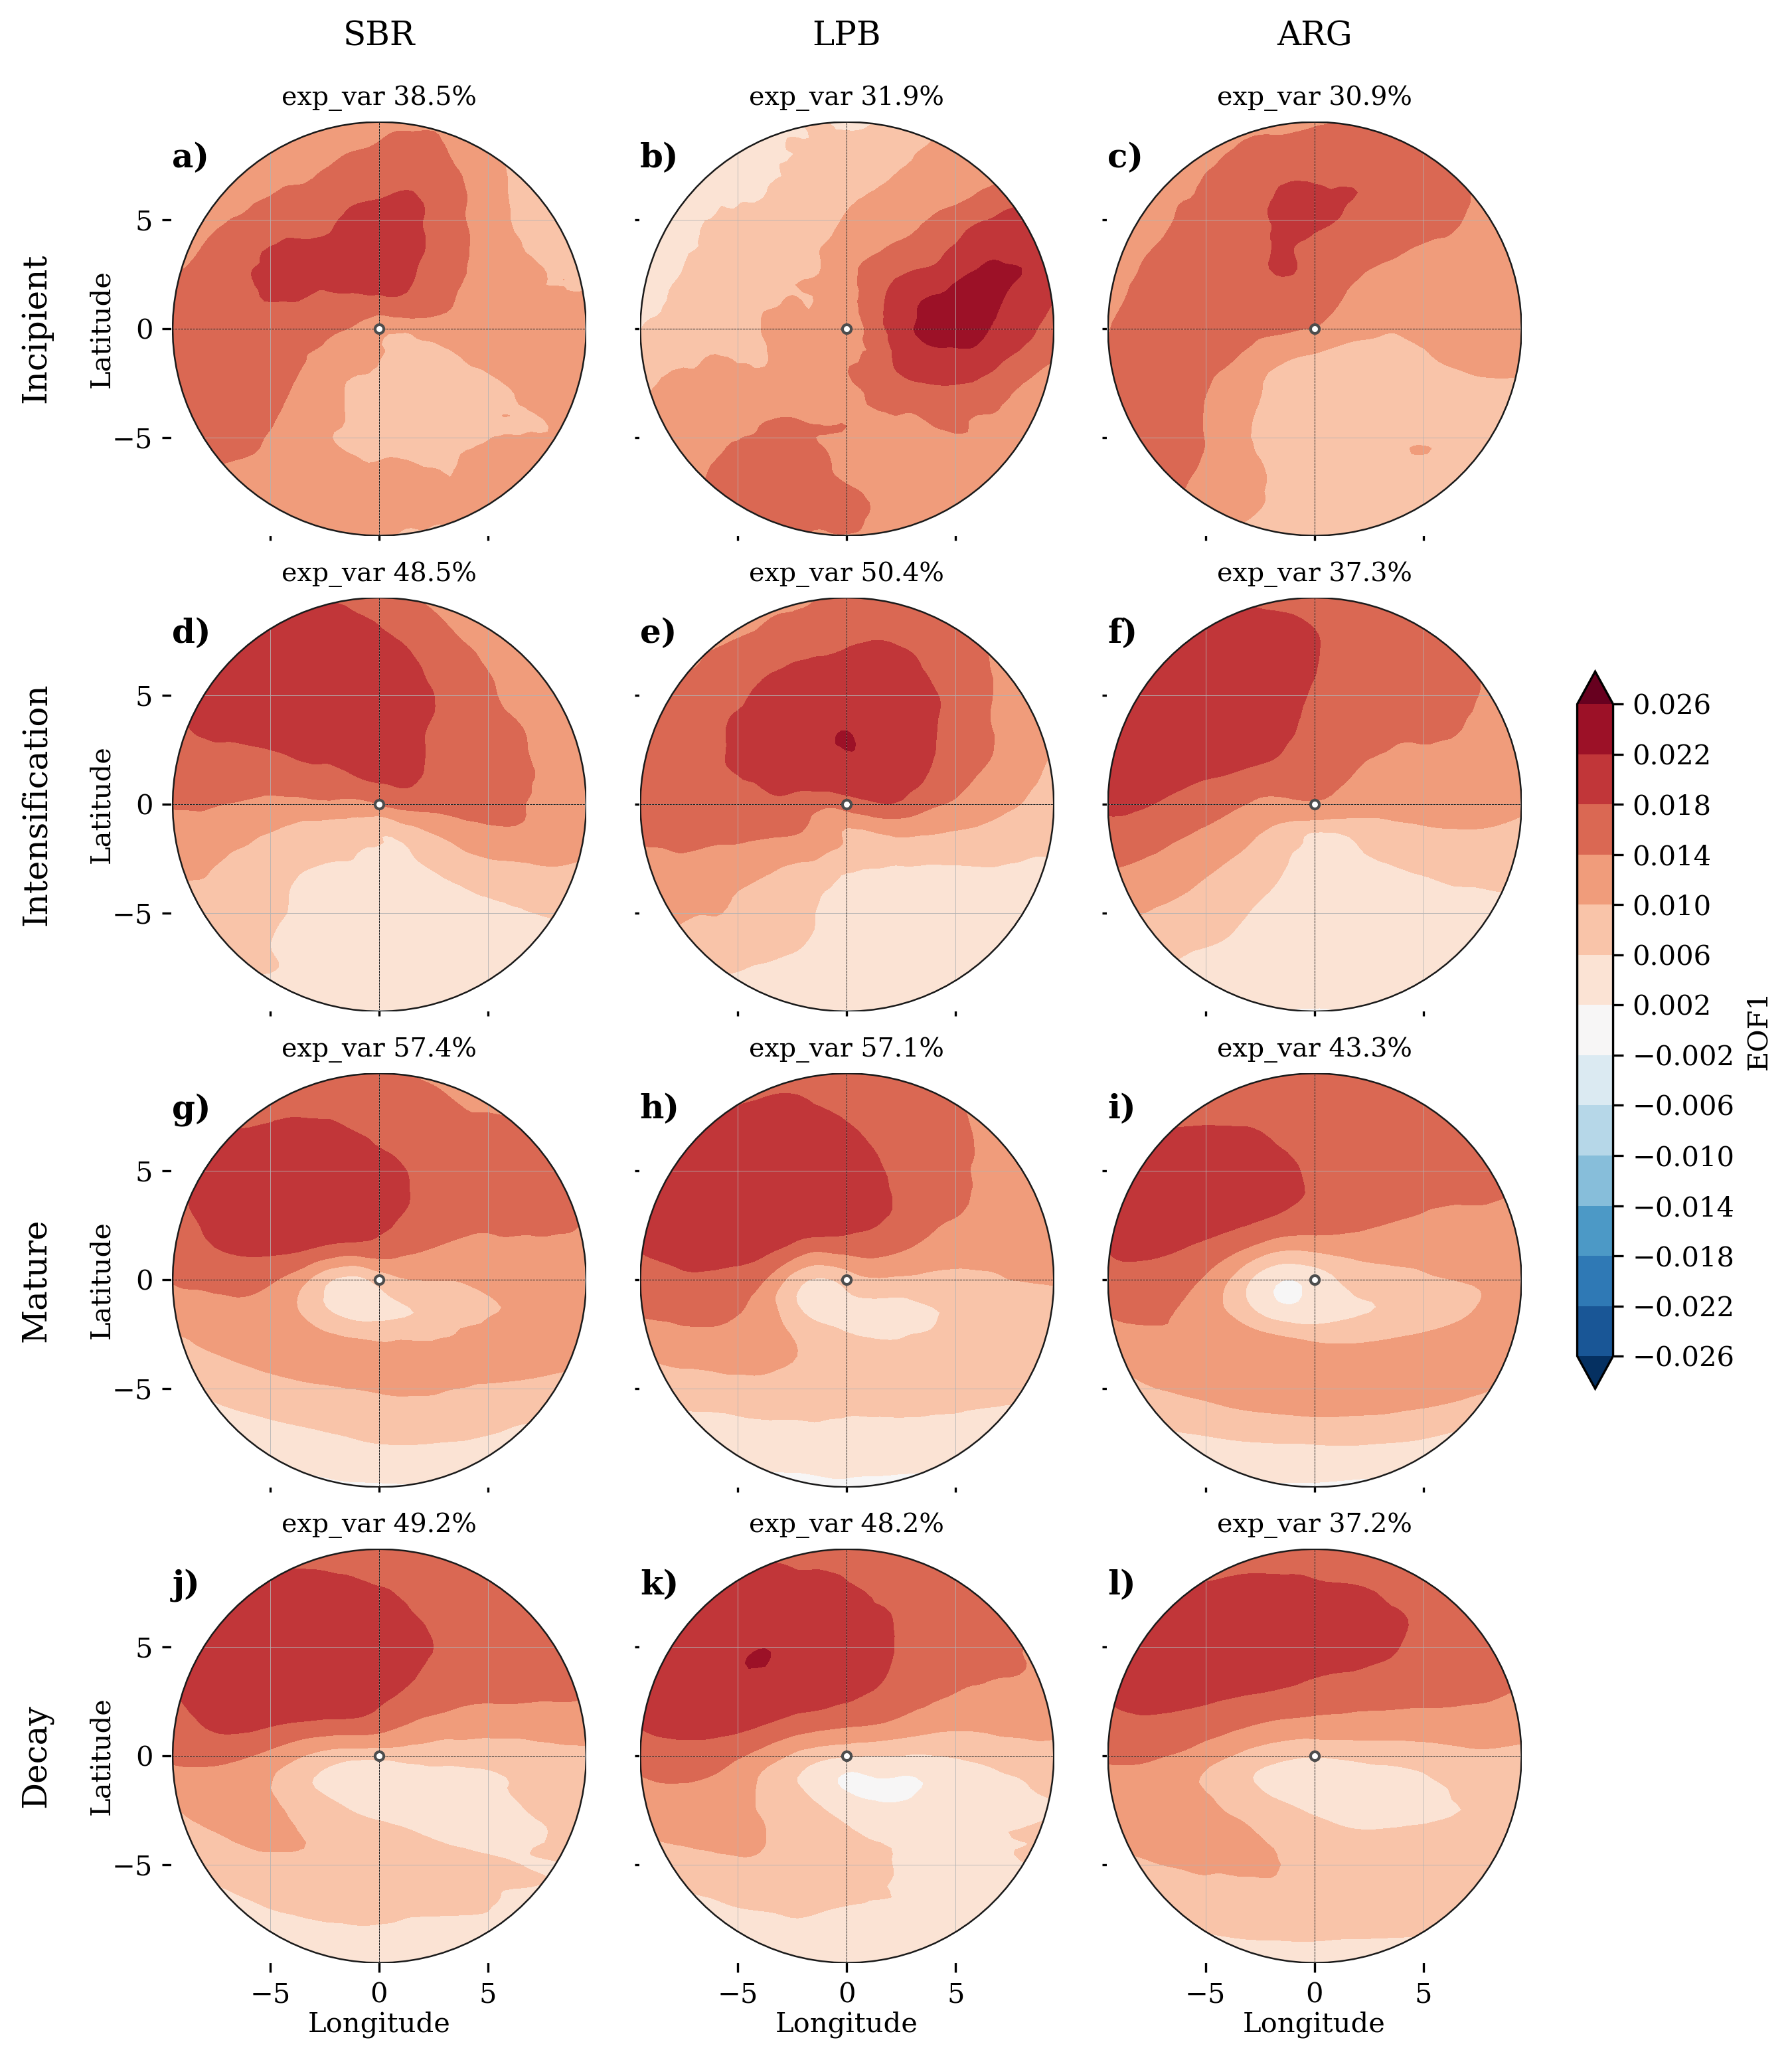
\includegraphics[width=\textwidth]{images/w10/pca1_wind10_global_fasesxreg.png}
\caption[EOF1 de la magnitud del viento a 10 metros - Población Global]{Primer modo espacial (EOF1) de la magnitud del viento a 10 metros para la Población Global de referencia. Los paneles (a-c) corresponden a la fase incipiente (Ic) para las regiones SBR, LPB y ARG, respectivamente; (d-f) a la intensificación (It); (g-i) a la madurez (M); y (j-l) al decaimiento (D). El título de cada panel indica el porcentaje de varianza explicada (\textit{exp\_var}) por este modo dominante. Los colores cálidos (fríos) representan anomalías positivas (negativas) de la estructura del viento relativo al centro del ciclón en un dominio de $20^{\circ} \times 20^{\circ}$.}
\label{fig:eof1_wind10_global}
\end{figure}

La Figura \ref{fig:eof1_wind10_global} presenta el primer modo de las Funciones Ortogonales Empíricas (EOF1) del campo de viento a 10 metros de altura, obtenido mediante la descomposición de la varianza total espacial sobre el dominio lagrangiano centrado en el ciclón. Este análisis se aplica sobre la Población Global (población de referencia) y se encuentra estratificado por región de ciclogénesis y fase de desarrollo, permitiendo aislar la estructura espacial más recurrente o el patrón dominante de fluctuación de los vientos superficiales a lo largo del ciclo de vida. Los mapas de los modos espaciales correspondientes a los estratos de menor intensidad (p10 y p50) se documentan en el Apéndice \ref{apendice:eof_wind10} para referencia complementaria.

Tal como se evidenció en el fraccionamiento de energía (Sección \ref{sec:var_exp_wind10}), el patrón EOF1 global domina ampliamente la varianza del sistema. Morfológicamente, rige una estructura dipolar de gran escala orientada meridionalmente. Durante la intensificación (d, f) y madurez (g, i) en SBR y ARG, se observan anomalías negativas extendidas al norte del centro (tonos azules, $-0.01$ a $-0.02$) y anomalías positivas marcadas al sur (tonos rojos, $+0.02$ a $+0.03$). La región LPB en intensificación (e) muestra un patrón morfológicamente distinto, con un núcleo anómalo positivo centralizado. Finalmente, en la fase de decaimiento (j, k, l), el dipolo se homogeneiza y adopta una disposición estrictamente zonal en todas las regiones, separando el dominio en una mitad norte negativa y una mitad sur fuertemente positiva.

La presencia de este dipolo norte-sur de gran escala en la población media, sumado a su alta varianza explicada, indica que la principal fuente de variabilidad en el viento de los ciclones típicos está dictada por su interacción con el flujo zonal de fondo (los vientos del oeste de latitudes medias) y las fluctuaciones del gradiente latitudinal de temperatura. Como detalla \citet{hannachi2007empirical}, la emergencia de una estructura dipolar dominante (EOF1) constituye la firma matemática que representa el desplazamiento posicional de una corriente. Físicamente, en el Hemisferio Sur, esto se traduce en desplazamientos de la latitud relativa de las corrientes en chorro en la alta troposfera. De acuerdo con \citet{hoskins2005new} y \citet{dossantos2023response}, la evolución estructural de los ciclones ordinarios depende fuertemente de este acoplamiento baroclínico profundo; por lo tanto, las anomalías capturadas por la EOF1 reflejan cómo el sistema expande o contrae su campo de viento en respuesta a la posición del chorro. 
% CITA TEXTUAL HANNACHI (2007): "Often, a dipole pattern in the first EOF represents a spatial shift or translation of a dominant atmospheric feature..."
% CITA TEXTUAL HOSKINS (2005) / DOS SANTOS (2023): 

El hecho de que las anomalías positivas de este dipolo se concentren marcadamente al sur del centro (tonos rojos en d, f, g, i) responde a la asimetría térmica característica de los sistemas del Atlántico Sur. Tal como describen \citet{sinclair1997objective} y \citet{reboita2010south}, a medida que los ciclones se intensifican y ganan latitud, el gradiente horizontal de presión tiende a maximizarse en su sector austral (o polar) debido a la interacción de la circulación ciclónica con los anticiclones migratorios, acelerando los vientos en esa franja. 
% CITA TEXTUAL SINCLAIR (1997) / REBOITA (2010):
La excepción geométrica observada en la región LPB (e) durante su intensificación respalda esta dependencia de los forzantes físicos: de acuerdo con \citet{gramcianinov2019properties}, los sistemas en esta zona están fuertemente modulados en sus etapas iniciales por la influencia de la baja orográfica, lo que genera una varianza del viento anclada a forzantes topográficos centralizados, retrasando temporalmente la imposición del dipolo zonal de gran escala. Finalmente, en el decaimiento, cuando la baroclinicidad se agota y el vórtice se debilita, la estructura circulatoria propia del ciclón pierde definición y la variabilidad queda completamente subyugada a los desplazamientos del gradiente de presión meridional del entorno sinóptico subyacente.
% CITA TEXTUAL GRAMCIANINOV (2019): "LA PLATA [LPB] cyclones development is influenced by an orographic low in their early stages..."

La extracción de este patrón univariado cumple la función de establecer la línea base de variabilidad estructural para el ciclón extratropical promedio. Identificar que la fluctuación principal en sistemas ordinarios obedece a un dipolo meridional permite separar matemáticamente las alteraciones inducidas por el entorno de aquellas generadas por la propia dinámica interna del vórtice. Este marco de referencia es instrumental para evaluar si los eventos extremos manifiestan modos espaciales organizativos diferentes o simplemente amplifican la señal de la población media.


\section{Patrones dominantes de variabilidad del viento a 10 metros: EOF1 Subconjunto extremo (p90)}\label{sec:eof1_wind10_p90}

\begin{figure}[htbp]
\centering
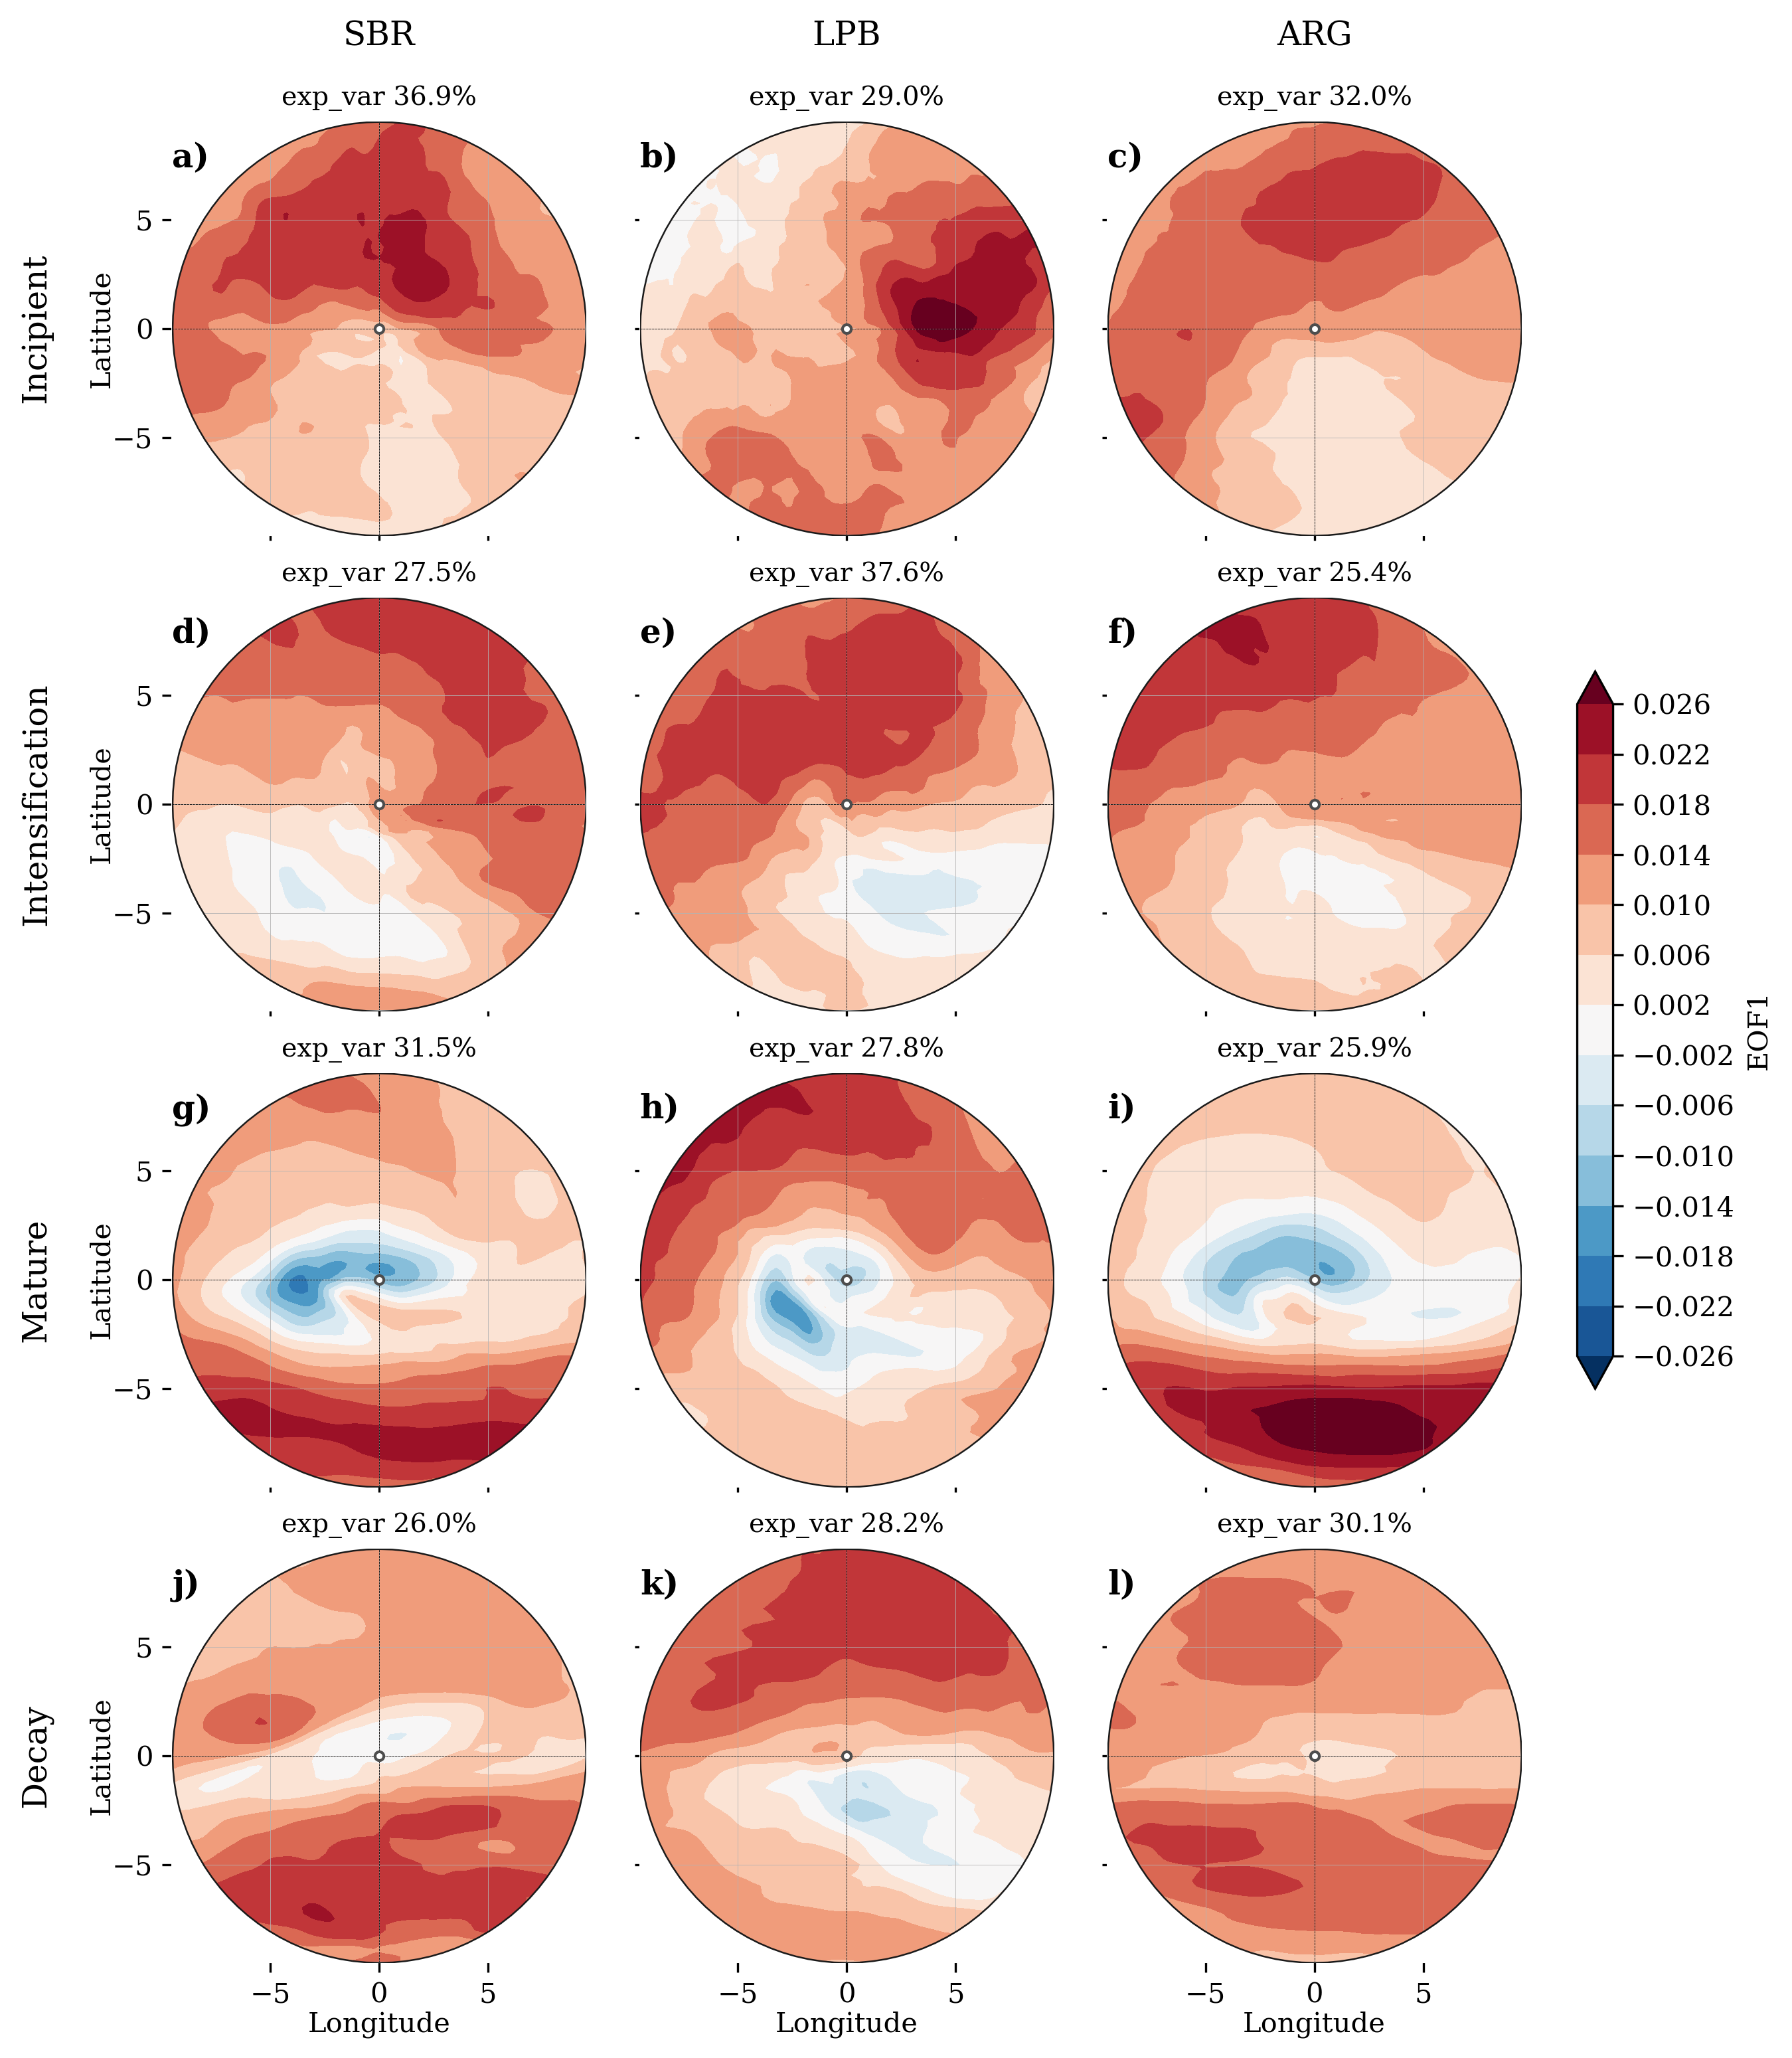
\includegraphics[width=\textwidth]{images/w10/pca1_wind10_p90_fasesxreg.png}
\caption[EOF1 de la magnitud del viento a 10 metros - Subconjunto p90]{Primer modo espacial (EOF1) de la magnitud del viento a 10 metros para el subconjunto de ciclones intensos (p90). La disposición de los paneles (a-l) por región de ciclogénesis (columnas) y fase evolutiva (filas) es idéntica a la Figura \ref{fig:eof1_wind10_global}. Se detalla la varianza explicada (\textit{exp\_var}) en cada panel y la barra de color estandarizada para evaluar las diferencias en las firmas espaciales de los eventos extremos frente al comportamiento climatológico.}
\label{fig:eof1_wind10_p90}
\end{figure}

La Figura \ref{fig:eof1_wind10_p90} ilustra la primera Función Ortogonal Empírica (EOF1) calculada exclusivamente a partir de los campos espaciales del subconjunto de ciclones extremos (percentil 90). Este análisis descompone el campo de viento relativo a 10 metros para aislar las fluctuaciones dominantes en los sistemas que, durante su ciclo vital, registraron los mínimos absolutos de vorticidad dentro del primer decil de la distribución. El resultado representa los modos de variabilidad intrínseca más característicos de los sistemas con mayor severidad dinámica, desglosados por fase de vida y zona de origen.

Tal como se anticipó en el fraccionamiento de la varianza (Sección \ref{sec:var_exp_wind10}), la proporción de energía capturada por el modo EOF1 en los sistemas extremos se reduce drásticamente frente a la población global, oscilando entre el $25.4\%$ y el $37.6\%$. En consonancia con esta caída, su topología difiere sustancialmente del dipolo zonal suave, mostrando firmas espacialmente complejas e hiperlocalizadas. En la fase de intensificación de SBR (d), emerge una fuerte anomalía positiva elongada hacia el suroeste (rojo oscuro, $>+0.03$). Más destacable es el comportamiento en madurez (g, h, i): LPB (h) exhibe un dipolo fuertemente inclinado con un núcleo positivo sumamente intenso y compacto justo al sur-sureste del centro, mientras que ARG (i) desarrolla un patrón tripolar complejo, con una marcada anomalía negativa en el núcleo rodeada de bandas de variabilidad positiva al sur. En el decaimiento (j, k, l), aunque retorna una estructura pseudozonal, los gradientes anómalos son notablemente más estrechos y confinados cerca del núcleo en comparación con la relajación expansiva observada en la población general.

La quiebra del patrón dipolar simple y la hiperlocalización de las anomalías son la manifestación espacial de la fragmentación de energía multiescalar discutida previamente. Físicamente, esto confirma que en los eventos extremos la intensa circulación cerrada de mesoescala domina sobre el flujo de fondo. El núcleo compacto y potente observado en la madurez de LPB (h) evidencia variabilidad en la posición exacta y severidad de estructuras mesoescalares. De acuerdo con el marco dinámico documentado por \citet{clark2005sting} y \citet{han2025system}, la hiperconcentración de vientos en los sectores posteriores y polares de ciclones profundos es la firma espacial de la cinta transportadora fría (\textit{cold conveyor belt}) y de procesos de fractura frontal rápida impulsados por altas tasas de vorticidad. Por otro lado, en ARG (i), la aparición de un patrón tripolar con una anomalía negativa central durante la madurez indica fluctuaciones en el tamaño o intensidad del "ojo" o seclusión cálida (\textit{warm seclusion}). Como detallan \citet{schultz2021antecedents} y \citet{reboita2022from}, la formación de esta seclusión cálida en el núcleo, rodeada por un anillo de vientos huracanados, es el rasgo evolutivo culminante del modelo conceptual de Shapiro-Keyser, una vía de desarrollo característica de ciclones con alta organización baroclínica y fuerte interacción con flujos anómalos en altas latitudes.
% CITA TEXTUAL CLARK (2005) / HAN (2025): 
% CITA TEXTUAL SCHULTZ (2021) / REBOITA (2022): "The Shapiro-Keyser cyclone model... features a wrapping around of the bent-back front to form a warm-core seclusion of post-cold-frontal air."

La cuantificación de estos modos revela una conclusión central: un ciclón extremo no es equivalente a un ciclón ordinario escalado linealmente, sino que su severidad dinámica modifica de raíz la arquitectura del sistema. Como enfatizan \citet{corner2025classification} y \citet{eisenstein2023identification}, la severidad del viento no depende únicamente de la profundidad sinóptica, sino de la manifestación de estas características mesoescalares. Identificar estas firmas asimétricas y compactas es clave para la meteorología operativa aplicada, ya que demuestra que la variabilidad de los vientos más destructivos se rige por procesos internos al vórtice, lo cual exige modelos de pronóstico capaces de resolver la dinámica estructural fina en los cuadrantes inmediatos al centro del ciclón.
% CITA TEXTUAL CORNER (2025) / EISENSTEIN (2023): 

% ==============================================================================
\subsection{Significancia espacial de los patrones en la fase de madurez}\label{subsec:res_significancia_madurez}

Para discriminar entre señales físicas robustas y fluctuaciones estocásticas propias del remuestreo, se evaluó la significancia estadística de los autovectores espaciales mediante el método Bootstrap-$t$ (Sección \ref{subsec:bootstrap_significancia}). La Figura \ref{fig:xeof_madurez_global} documenta los tres primeros modos (EOF1--EOF3) y sus respectivas series temporales (PC1--PC3) para la Población Global en fase de madurez, mientras que la Figura \ref{fig:xeof_madurez_p90} presenta el análisis equivalente para el subconjunto extremo (p90). El achurado ($\backslash\backslash\backslash$) delimita las áreas donde las cargas espaciales resultaron estadísticamente significativas al 95\% de confianza.

\begin{figure}[htbp]
\centering
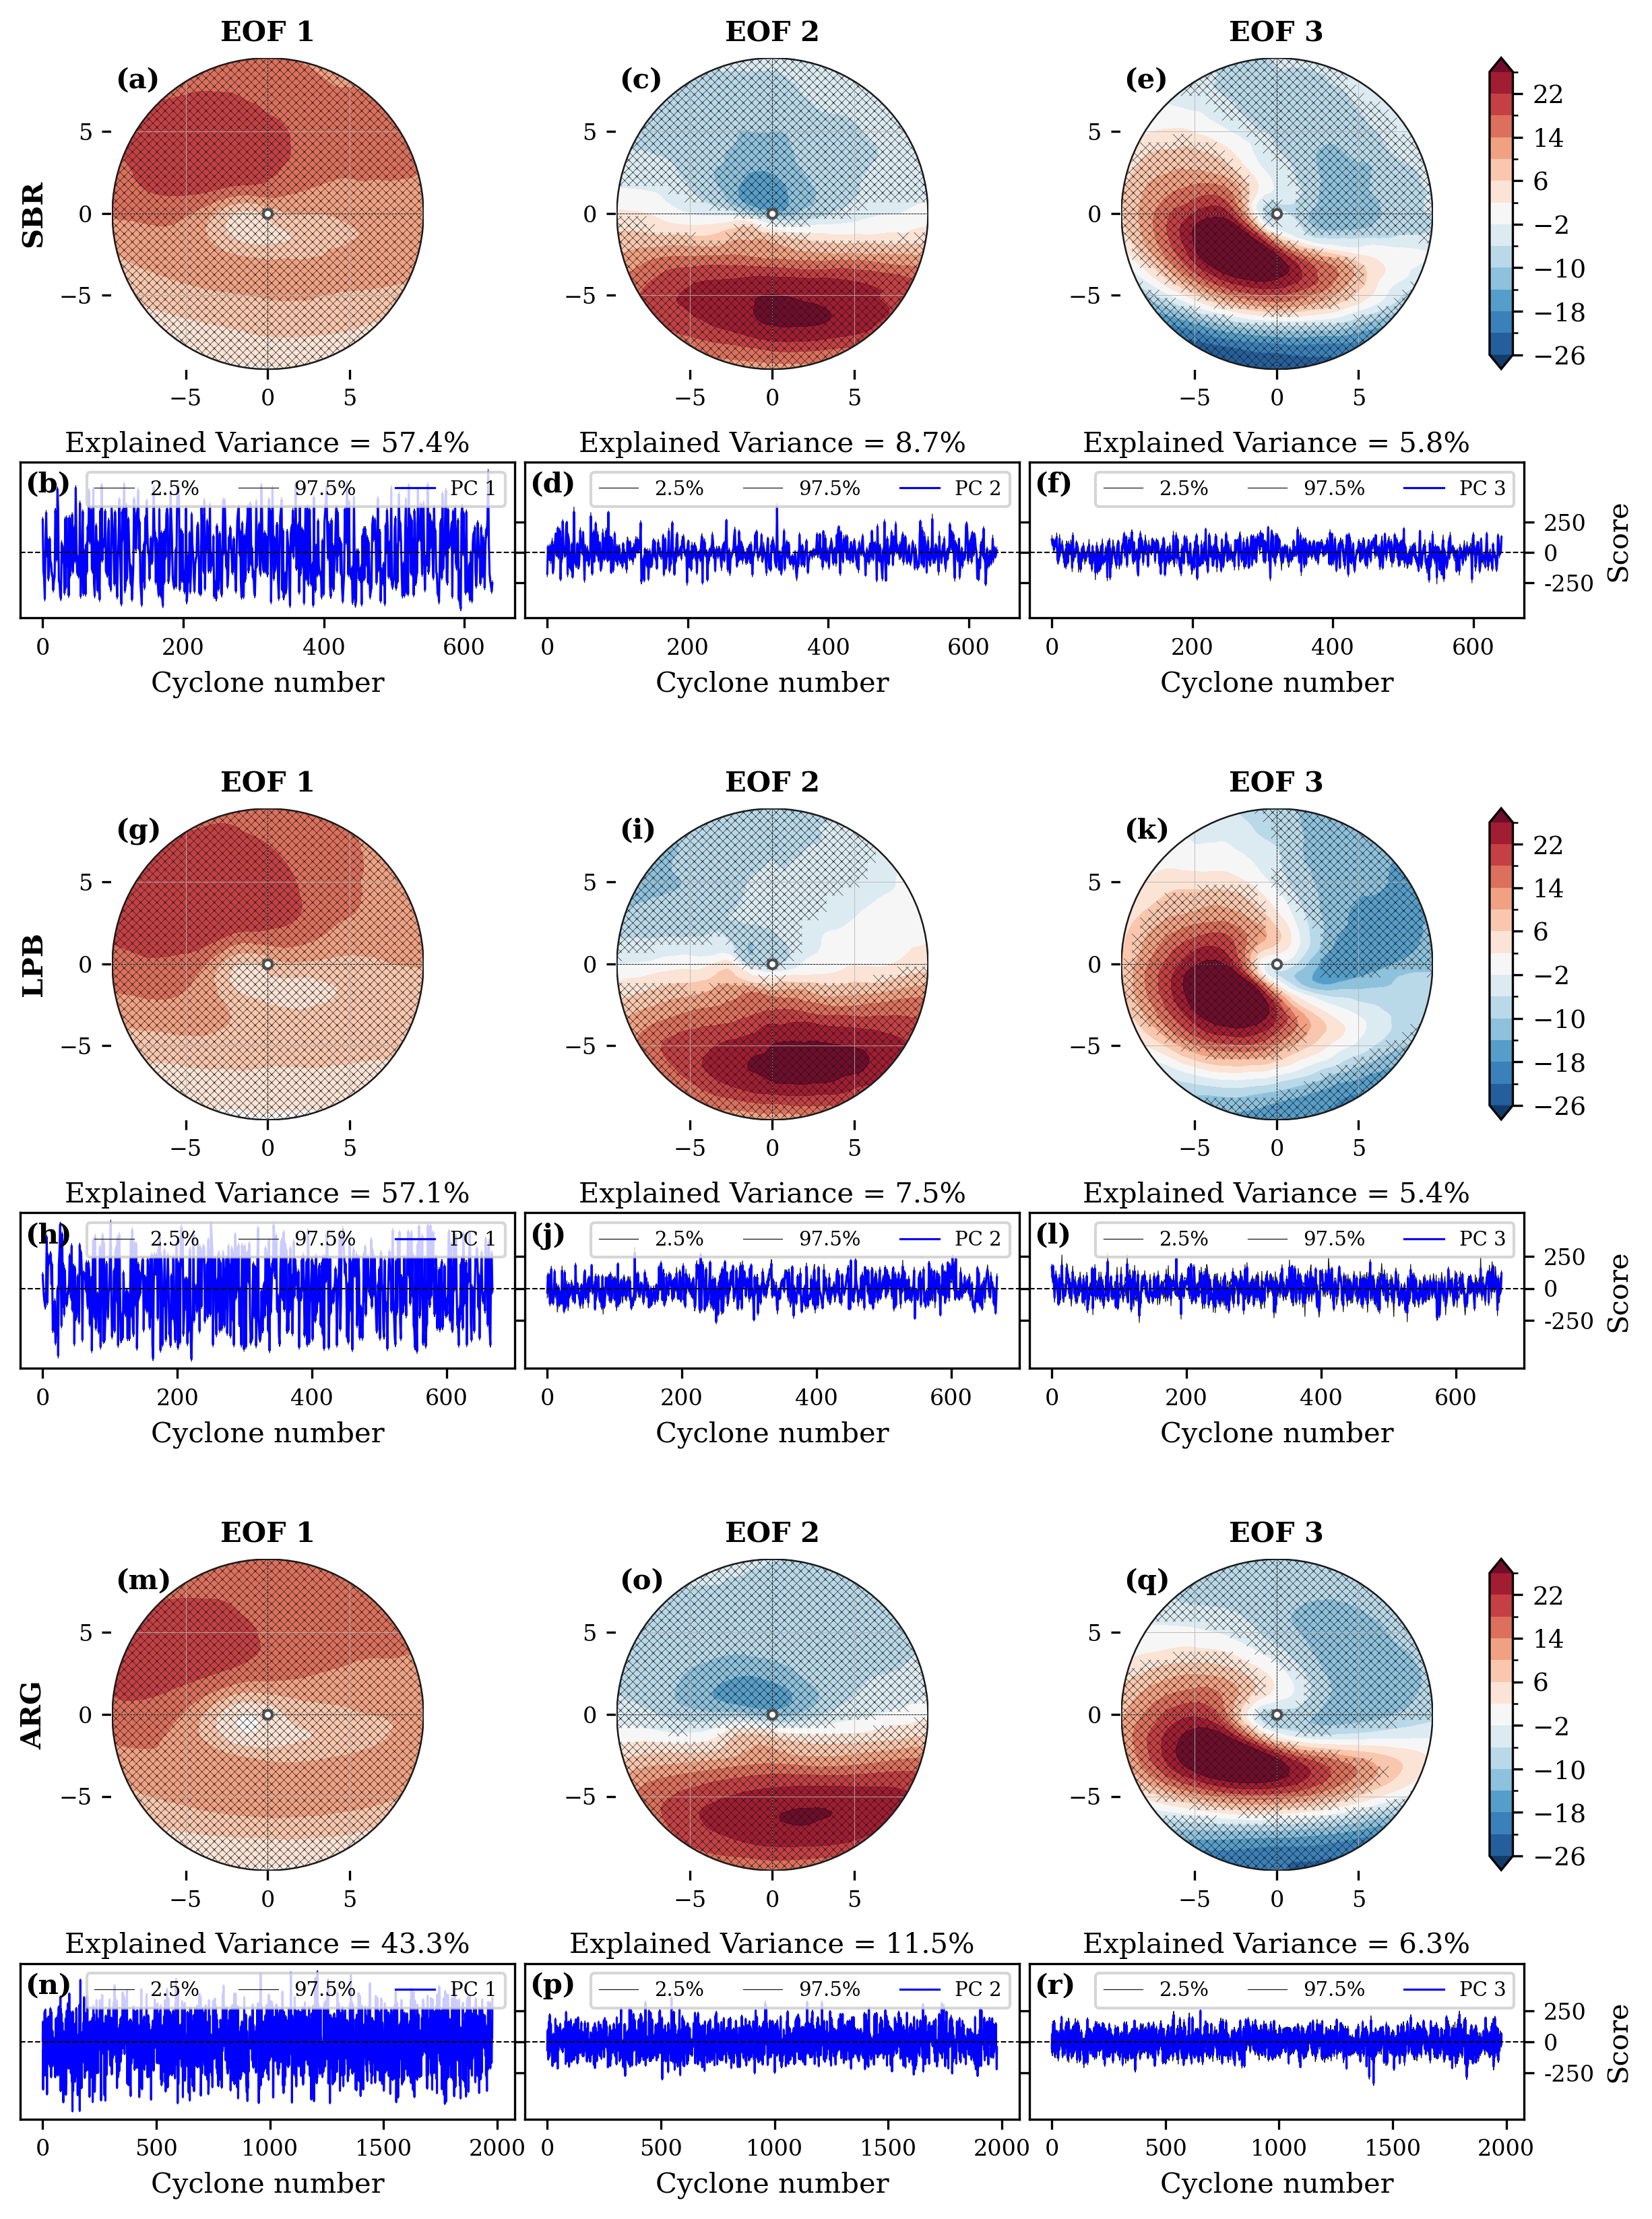
\includegraphics[width=\textwidth]{images/w10/xeof_global_wind10_mature.png}
\caption[Significancia espacial de los EOFs en fase de madurez - Población Global]{Descomposición EOF del viento a 10 m para la Población Global en fase de madurez. Paneles (a, c, e): mapas de los tres primeros modos espaciales (EOF1--EOF3) con achurado indicando significancia estadística al 95\% (test Bootstrap-$t$). Paneles (b, d, f): series temporales correspondientes de las Componentes Principales (PC1--PC3). La línea gris delimita los percentiles 2.5 y 97.5 de la distribución bootstrap.}
\label{fig:xeof_madurez_global}
\end{figure}

\begin{figure}[htbp]
\centering
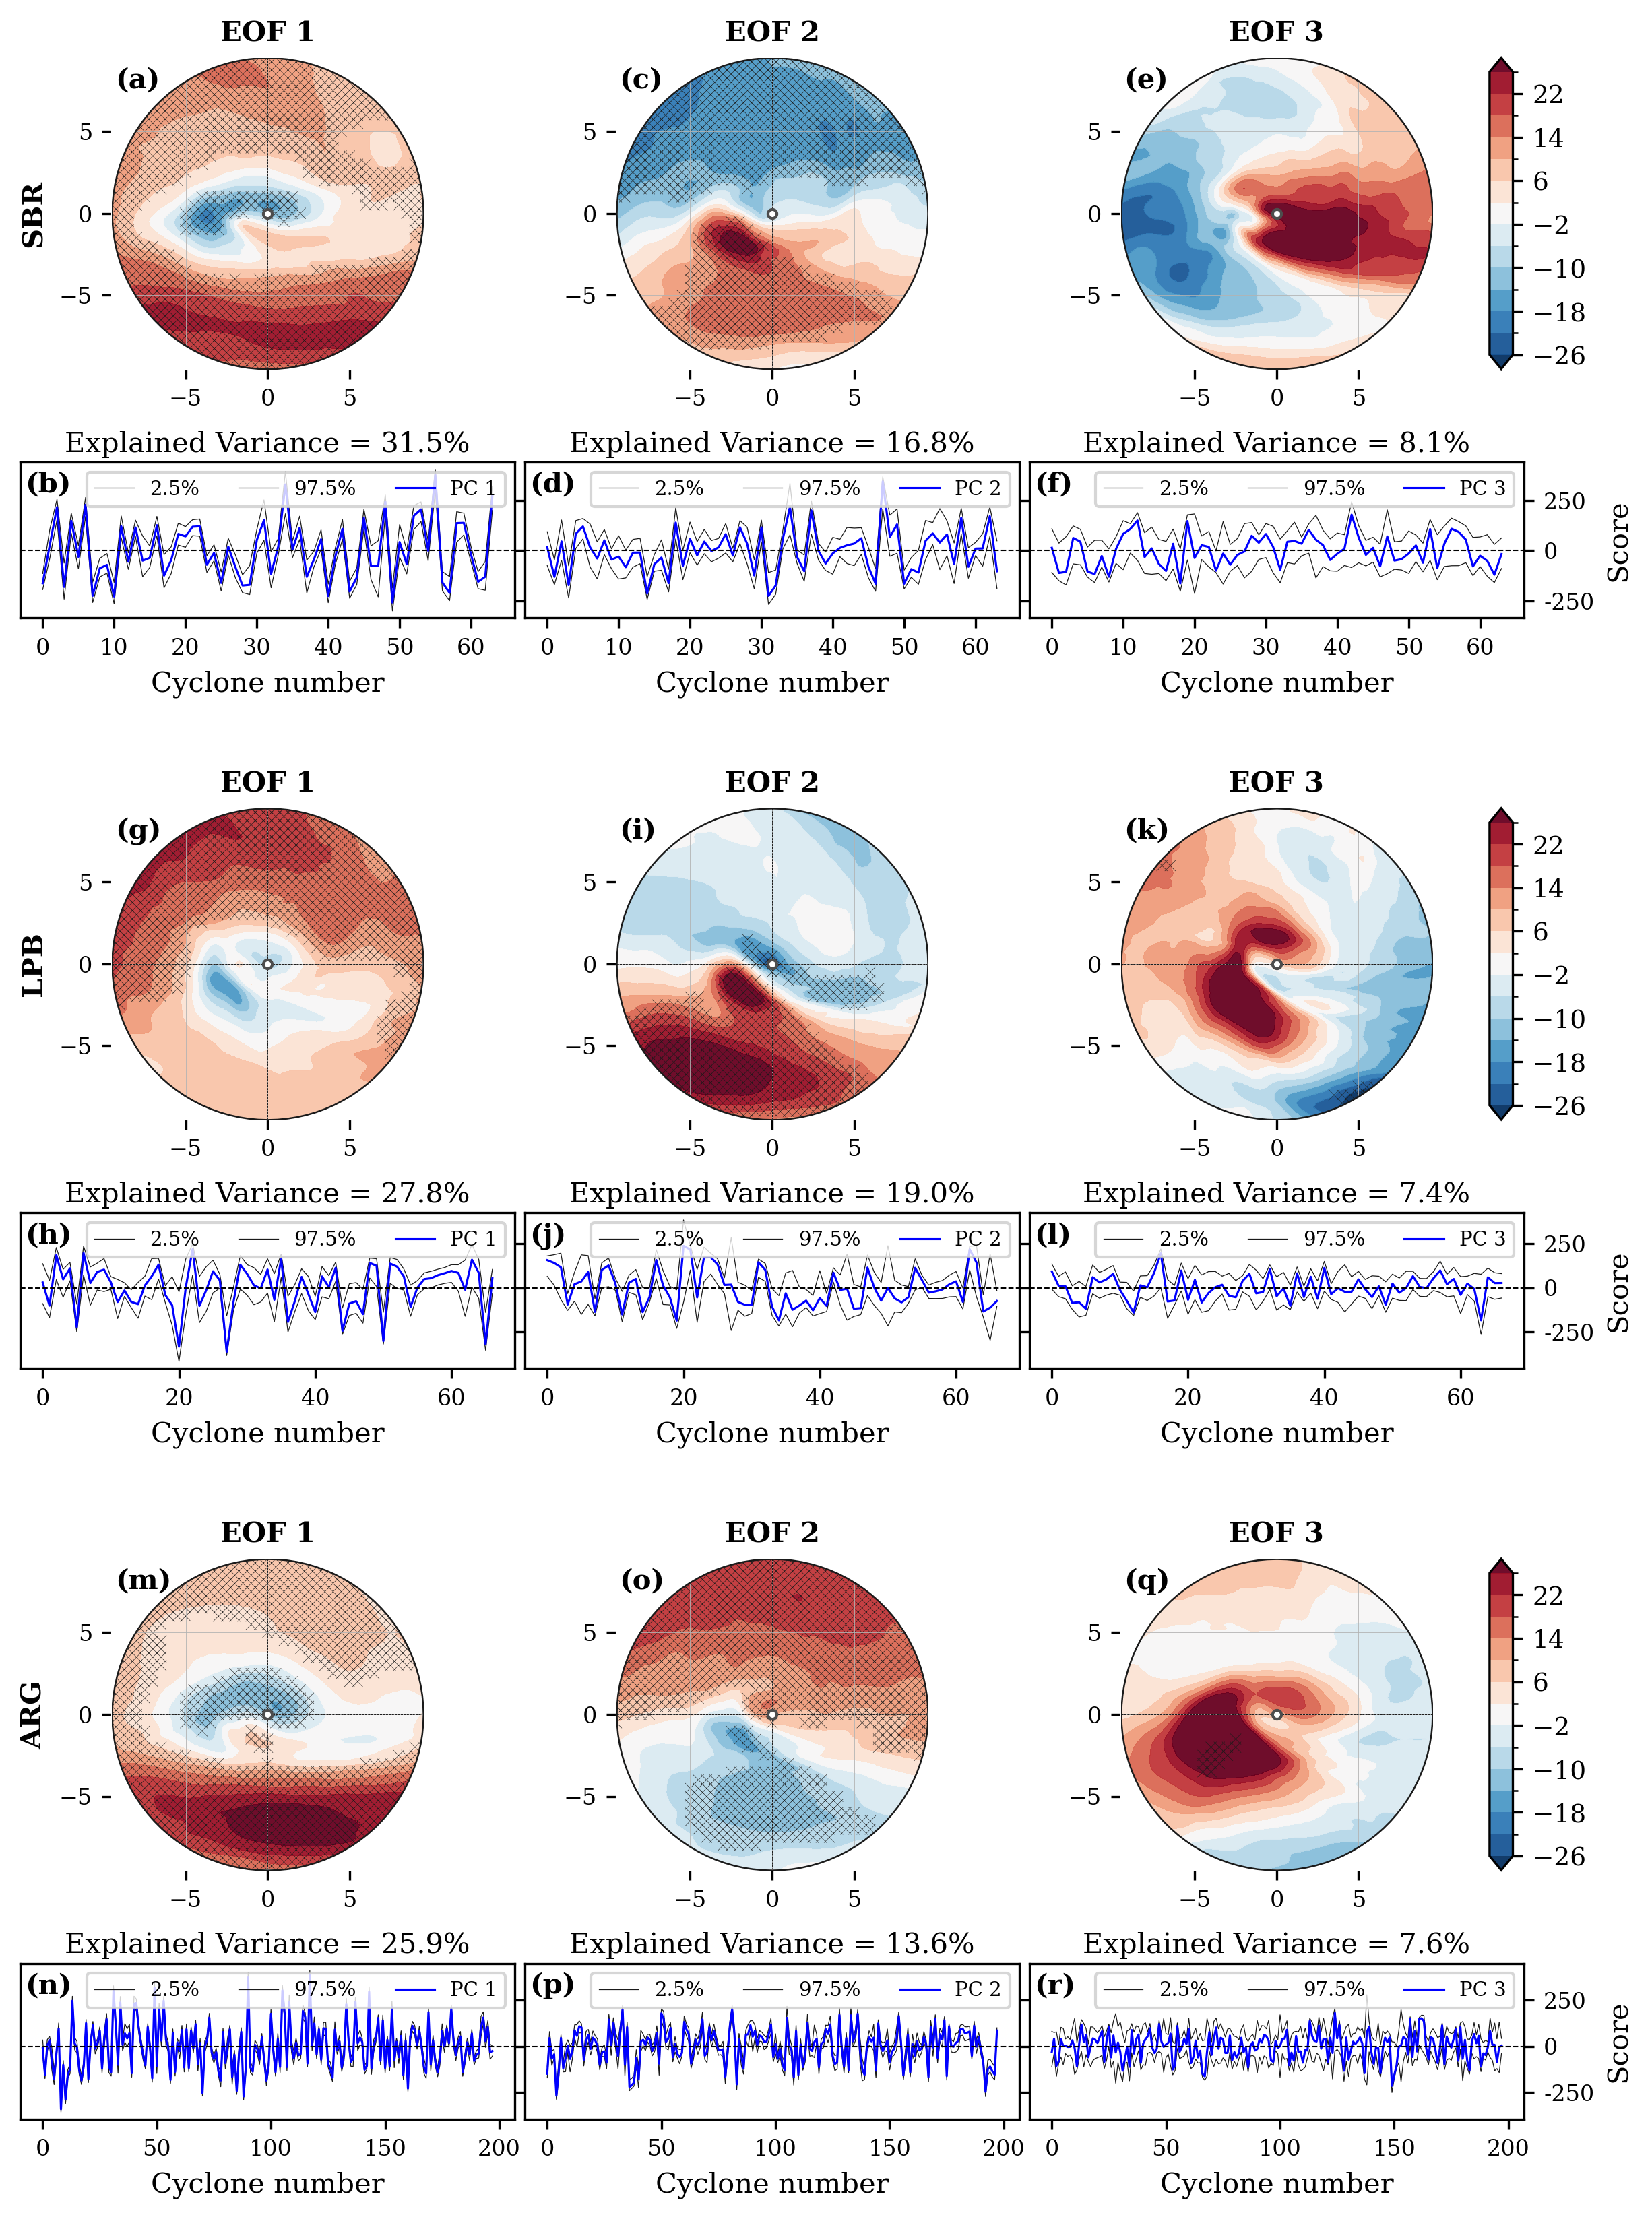
\includegraphics[width=\textwidth]{images/w10/xeof_p90_wind10_mature.png}
\caption[Significancia espacial de los EOFs en fase de madurez - Subconjunto p90]{Descomposición EOF del viento a 10 m para el subconjunto extremo (p90) en fase de madurez. La disposición de paneles es idéntica a la Figura \ref{fig:xeof_madurez_global}.}
\label{fig:xeof_madurez_p90}
\end{figure}

En la Población Global (Figura \ref{fig:xeof_madurez_global}), el modo dominante (EOF1) exhibe áreas de significancia estadística que abarcan prácticamente todo el dominio, particularmente en los sectores norte y sur donde se localizan los máximos del dipolo baroclínico (paneles a, g, m). Esta extensión espacial de la significancia indica que el patrón dipolar no es un artefacto de la muestra, sino una característica física estable y reproducible de los ciclones maduros. Consistente con el alto porcentaje de varianza explicada (43--57\%), las series de PC1 (paneles b, h, n) muestran amplitudes que oscilan ampliamente y dominan sobre las fluctuaciones de PC2 y PC3, las cuales permanecen confinadas dentro de los límites de confianza (líneas grises) y representan meramente ruido de fondo o variabilidad intra-sistémica menor.

Por el contrario, en el subconjunto extremo (Figura \ref{fig:xeof_madurez_p90}), las áreas significativas del EOF1 experimentan una dramática contracción hacia núcleos compactos próximos al centro del vórtice (paneles a, g, m). En SE-BR y LPB, la significancia se restringe a pequeños parches alrededor del núcleo y el flanco sur, mientras que en ARG el patrón tripolar presenta significancia únicamente en el anillo periférico sur. Esta contracción espacial confirma que, en ciclones intensos, el modo dominante pierde coherencia espacial fuera del núcleo inmediato; la estructura del viento ya no está gobernada por un gradiente sinóptico extendido, sino por procesos de mesoescala localizados (seclusiones térmicas, jets de bajo nivel) que varían sustancialmente entre eventos individuales.

Más crítico aún es el comportamiento de las series temporales en el grupo p90 (paneles b, d, f y h, j, l). A diferencia del grupo Global donde PC2 y PC3 son residuales, aquí las amplitudes de PC2 (línea azul en paneles d, j) y PC3 (paneles f, l) frecuentemente superponen o incluso exceden los rangos de PC1, cruzando los límites de confianza de manera sistemática. Esto demuestra estadísticamente que los modos secundarios han dejado de ser ``ruido'' para convertirse en portadores de varianza física significativa. La competencia energética entre múltiples PCs refleja la fragmentación dinámica del campo de viento: cuando un ciclón alcanza severidad extrema, su estructura cinemática ya no puede describirse mediante un único patrón espacial dominante, sino que requiere la superposición de varios modos ortogonales competitivos.

La implicación meteorológica es profunda. La contracción de las áreas significativas en el grupo p90 indica que la predictibilidad espacial del campo de viento se reduce drásticamente en ciclones extremos. Mientras que en sistemas ordinarios podemos confiar en que el patrón dipolar extendido representará fielmente la distribución de vientos (alta significancia espacial), en sistemas severos solo el núcleo inmediato del vórtice presenta una señal robusta; los flancos y cuadrantes periféricos están dominados por variabilidad estocástica o estructuras transitorias de mesoescala que escapan al primer modo. Esto valida la necesidad de incluir EOF2 y EOF3 en cualquier reconstrucción o pronóstico de campos de viento para ciclones intensos, ya que el primer modo por sí solo ya no captura adecuadamente la estructura física del sistema.

% ==============================================================================
% ==============================================================================
% ==============================================================================
% ------------------------------------------------------------------------------
\subsection{Dinámica de las amplitudes modales (PC1)}\label{subsec:res_dinamica_pc1}
% ------------------------------------------------------------------------------

La fragmentación de la varianza y la contracción de las áreas significativas observadas en la fase de madurez (Sección \ref{subsec:res_significancia_madurez}) tienen su contraparte temporal en el comportamiento estadístico de las Componentes Principales. Mientras que en la Población Global la PC1 domina establemente la evolución del sistema —evidenciado por sus amplitudes superiores y áreas significativas extensas—, en los ciclones extremos la competencia entre múltiples modos ortogonales (Figura \ref{fig:xeof_madurez_p90}) se traduce en propiedades estadísticas distintivas: una correlación débil con el forzante sinóptico y distribuciones de probabilidad con colas pesadas que reflejan la bifurcación estructural de estos sistemas.

\input{tabelas_es/tab_momentos_global_w10.tex}

\subsubsection{Población Global: Convergencia hacia el patrón sinóptico dominante}

Las Tablas \ref{tab:momentos_global_w10} y \ref{tab:corr_global_w10} documentan las métricas estadísticas de la PC1 para la Población Global. Al evaluar la evolución de la población media, la distribución de la PC1 exhibe una progresiva \textit{normalización} estructural. En las tres regiones (SE-BR, LPB y ARG), los valores de curtosis oscilan de forma consistente entre $-0.30$ y $-1.03$ durante la intensificación y madurez, evidenciando distribuciones platicúrticas sin colas extremas dominantes. Notablemente, el régimen transicional de LPB muestra la mayor variabilidad inicial (skewness $+0.99$, leptocurtosis $+1.32$ en fase incipiente), mientras que SE-BR y ARG presentan poblaciones más homogéneas desde etapas tempranas.

El rasgo evolutivo más contundente emerge en el acoplamiento con la vorticidad: en todas las cuencas, la correlación inicial —que oscila entre $-0.35$ (LPB) y $-0.57$ (SE-BR)— experimenta un \textit{fortalecimiento sistemático} hasta alcanzar valores excepcionales en la madurez ($-0.890$ en SE-BR, $-0.868$ en LPB y $-0.860$ en ARG), manteniéndose altos durante el decaimiento ($\rho < -0.75$).

Físicamente, este acoplamiento casi lineal (que explica hasta $r^2 \approx 0.79$ de la varianza en SE-BR) demuestra que, en los ciclones ordinarios, la variabilidad espacial del viento está gobernada directamente por el gradiente de presión a escala sinóptica. La progresiva simetrización de la distribución de PC1 (skewness tendiendo a cero) evidencia que, a medida que el vórtice se intensifica, los campos de viento convergen hacia una configuración prototípica bien definida, dominada por el primer modo de variabilidad.

\input{tabelas_es/tab_corr_global_w10.tex}

Esta convergencia implica que, para la mayoría de los ciclones, la estructura espacial del viento no es arbitraria, sino que se organiza en torno a un patrón coherente (EOF1). La severidad extrema rompe dicha organización, permitiendo que el sistema explore múltiples configuraciones espaciales válidas (fragmentación multiescalar).

La diferencia regional clave reside en la velocidad de esta convergencia: mientras SE-BR exhibe un acoplamiento fuerte desde etapas incipientes (consistente con su naturaleza híbrida donde la convección organiza rápidamente el campo de viento), LPB requiere la fase de intensificación para alcanzar dicho estado (pasando de $\rho = -0.35$ a $-0.71$), reflejando su carácter transicional donde la organización frontal emerge solo cuando el forzante baroclínico se establece con suficiente intensidad.

Establecer esta línea base cinemática es vital para la meteorología sinóptica, ya que valida estadísticamente que los modelos de desarrollo de gran escala son plenamente predictivos para la mayoría de los ciclones. Confirma que, en sistemas de intensidad regular, es posible inferir con alta confianza la magnitud espacial de la circulación superficial observando únicamente la profundidad del núcleo de baja presión.

\subsubsection{Subconjunto Extremo (p90): Desacoplamiento estructural y bifurcación dinámica}

Las Tablas \ref{tab:momentos_p90_w10} y \ref{tab:corr_p90_w10} exponen los parámetros estadísticos para el estrato de ciclones más intensos (p90). La dinámica de los eventos extremos rompe drásticamente con la linealidad observada en la climatología. En lugar de intensificarse hacia la madurez, la correlación entre PC1 y vorticidad exhibe un colapso estructural en las regiones baroclínicas: en ARG cae progresivamente desde $-0.43$ (incipiente) hasta un mínimo de $-0.26$ en madurez, mientras que LPB y SE-BR muestran correlaciones estancadas o en descenso ($-0.37$ y $-0.44$, respectivamente). 

Este colapso correlacional es consistente con la pérdida de significancia espacial observada en el modo dominante (Figura \ref{fig:xeof_madurez_p90}, paneles a, g, m): cuando el patrón espacial solo es robusto en el núcleo inmediato del vórtice pero no en los flancos (como documentó el test Bootstrap-$t$ en la sección anterior), su amplitud temporal (PC1) deja de escalar coherentemente con la intensidad sinóptica global ($\zeta_{850}^{min}$).

\input{tabelas_es/tab_momentos_p90_w10.tex}

Paralelamente, las distribuciones de probabilidad revelan una \textit{heterogeneización} marcada. LPB exhibe leptocurtosis ($\gamma_2 = +0.96$) y fuerte asimetría negativa ($\gamma_1 = -0.88$) durante la intensificación, indicando una población bimodal de configuraciones estructurales. SE-BR, por su parte, mantiene estabilidad durante el desarrollo pero exhibe una bifurcación extrema en el decaimiento: una leptocurtosis explosiva ($\gamma_2 = +3.95$) con skewness positivo ($+1.15$), evidenciando que los ciclones intensos no siguen un único camino estructural hacia la disipación.

Físicamente, la caída del acoplamiento en la fase de madurez constituye la manifestación empírica del desacoplamiento mesoescalar. Cuando un ciclón se profundiza hasta valores extremos, la organización del viento a 10 metros deja de obedecer puramente al mínimo de vorticidad global y pasa a ser controlada por procesos secundarios: génesis de seclusiones cálidas en ARG, organización convectiva profunda independiente en SE-BR, o interacciones orográficas persistentes en LPB. 

La emergencia de curtosis positiva en LPB (intensificación/madurez) y SE-BR (decaimiento) demuestra que la severidad se alcanza a través de una \textit{diversidad de estructuras asimétricas} que el modo dominante no captura, generando colas pesadas de eventos atípicos. Sorprendentemente, el acoplamiento solo se recupera abruptamente durante el decaimiento (alcanzando $-0.74$ en ARG), sugiriendo que, una vez disipadas las anomalías térmicas de mesoescala (fricción y pérdida de gradiente), la circulación remanente vuelve a alinearse linealmente con el vórtice residual.

\input{tabelas_es/tab_corr_p90_w10.tex}

Este hallazgo cuantitativo constituye una demostración meteorológica de primer orden: prueba que alcanzar la severidad dinámica máxima induce un \textit{desacople temporal} crítico entre el campo de viento superficial y el centro de baja presión profundo durante la fase de madurez. Esto indica que parametrizar la evolución cinemática de un ciclón severo utilizando únicamente $\zeta_{850}$ o la presión central resultará insuficiente en el momento crítico de impacto, ya que la distribución de los vientos obedece a alteraciones internas de mesoescala que escapan de la linealidad sinóptica. 

La implicancia operacional es clara: los sistemas de alerta temprana requieren diagnósticos adicionales (temperatura del aire en seclusiones, tasas de precipitación convectiva, o análisis de estabilidad estática) para predecir los campos de viento extremo en ciclones profundos, particularmente en las regiones de LPB y ARG donde el desacoplamiento es más pronunciado.
% ==============================================================================
